%  A profile model for semi-analytical bathymetry from multispectral imagery.
%  MDPI Remote Sensing template (Definitions/mdpi.cls). Build: pdflatex twice.
%  Figures: validation/paper_profile.py figures (writes paper/msab_figures/).

\documentclass[remotesensing,article,submit,pdftex]{Definitions/mdpi}

\firstpage{1}
\makeatletter
\setcounter{page}{\@firstpage}
\makeatother
\pubvolume{1}
\issuenum{1}
\articlenumber{0}
\pubyear{2026}
\copyrightyear{2026}
\datereceived{ }
\daterevised{ }
\dateaccepted{ }
\datepublished{ }
\hreflink{https://doi.org/}

\Title{Semi-Analytical Bathymetry from Multispectral Imagery by Exact Depth Profiling}

\TitleCitation{Semi-Analytical Bathymetry from Multispectral Imagery by Exact Depth Profiling}

\Author{Sam Blake $^{1,}$*}

\AuthorNames{Sam Blake}

\AuthorCitation{Blake, S.}

\address{%
$^{1}$ \quad The University of Melbourne, Melbourne, Australia}

\corres{Correspondence: samuel.thomas.blake@gmail.com}

\abstract{Physics-based (semi-analytical) inversion of shallow-water reflectance was designed for hyperspectral data. Applied to four-band multispectral imagery such as Sentinel-2, the joint fit of water, bottom and depth is poorly posed: on real scenes its misfit is nearly flat in depth, so the result depends on the start and the optimiser rather than on the data. We derive a semi-analytical model for multispectral imagery from Lee's shallow-water reflectance model with three changes. First, the water is observed rather than fitted: each scene's deep-water reflectance is taken from its own optically deep pixels, which are found without soundings, and the attenuation follows by a quasi-analytical algorithm. Second, the bottom brightness and a per-scene offset enter linearly, so for every depth on a fixed grid they are solved exactly; the misfit profile in depth is then exact and its global minimum is found by construction. Third, a depth is reported only when the profile excludes both optically deep water and a clearly different depth. We validate the model against radiative-transfer simulations and, without soundings or a depth prior, against singlebeam surveys at four sites in Exmouth Gulf, Western Australia, using six Sentinel-2 scenes. Settings were tuned on training sites and tested once on held-out sites. Compared with the previous semi-analytical model, depths within tolerance rose from 6--23\% to 21--54\% of the surveyed cells at three sites, at about 500 times the speed, with better-calibrated uncertainties. The gains are confined to depths of 0--5\,m: deeper bottoms are reported too shallow or abstained from, and a product calibrated with soundings remains more accurate in deeper water.}

\keyword{satellite-derived bathymetry; semi-analytical model; Sentinel-2; multispectral; inverse problem; identifiability; optically deep water; uncertainty}

\begin{document}

\section{Introduction}

Satellite-derived bathymetry (SDB) estimates the depth of shallow water from the light reflected by the seabed. Empirical methods regress depth against band ratios or log-transformed reflectances~\cite{lyzenga1978,lyzenga2006,stumpf2003,caballero2019}, and so need soundings at every site and for every image. Physics-based methods instead invert a radiative-transfer model of the water column and the bottom for depth, water optical properties and bottom reflectance together~\cite{lee1998,lee1999,lee2001,mobley2005,brando2009,dekker2011}. Of these, the semi-analytical model of Lee et al.~\cite{lee1998,lee1999} (HOPE) has been the most widely adapted~\cite{wettle2006,klonowski2007,hedley2009,hedley2018}. It needs no soundings in principle, which is the reason to prefer it.

HOPE was designed for hyperspectral data. Lee and Carder~\cite{lee2002bands} found that about fifteen bands between 400 and 800\,nm suffice to separate water, bottom and depth. The freely available multispectral sensors that cover the world's coasts, Landsat~8 and Sentinel-2~\cite{drusch2012}, have four visible bands that reach the seabed. With four bands, a single-scene HOPE inversion has more unknowns than data. The photic model~\cite{blake2020} addressed this by assuming that depth and bottom are constant across several scenes (up to the tide) and that the water is constant over a small window around each pixel. Each scene then adds three water parameters for its four data, and the inversion becomes a non-linear least-squares problem with tens of parameters, solved by local optimisation from heuristic starts.

We built a four-tier benchmark to test that model (Section~\ref{sec:validation}). It showed two things. First, Lee's forward model is a good approximation of exact radiative transfer, with a median error of 2.4\%. Second, the inversion does not recover depth on real Sentinel-2 scenes without a depth prior. At Exmouth Gulf, with the true depth given as the starting point, the misfit at the true depth was no lower than at a wrong shallow depth (5.2\% against 5.1\% relative error). The misfit is nearly flat in depth because the scene water parameters, the bottom brightness and depth can trade against one another, and because the fit absorbs the forward model's own few-per-cent error into whichever parameter is freest. Once the misfit is flat in depth, no search strategy can recover depth, so the problem lies in how the model is posed.

In this paper we derive a semi-analytical model for multispectral imagery, the profile model, which keeps Lee's physics but changes what is fitted. The water is observed from each scene's optically deep pixels and not fitted to the pixel. The two remaining per-pixel unknowns other than depth, the bottom brightness and a per-scene offset, enter the model linearly and are solved exactly at every candidate depth. Depth, the only non-linear unknown, is searched exhaustively on a fixed grid, so the minimum of the misfit is global by construction. Finally, the profile of the misfit in depth decides whether a depth is reported at all. Section~\ref{sec:model} derives the model and lists every assumption it makes. Section~\ref{sec:data} describes the Exmouth Gulf case study and the validation design. The design separates tuning data from test data, and reports a held-out test run once. Section~\ref{sec:results} gives the results, including where the model fails, and Section~\ref{sec:discussion} discusses them.

\section{The Profile Model}\label{sec:model}

\subsection{Shallow-Water Reflectance}\label{sec:rt}

Let $R_\mathrm{rs}(\lambda)$ be the remote-sensing reflectance just above the surface and $r_\mathrm{rs}(\lambda)$ that just below it. For a flat surface and a near-nadir view~\cite{lee1999},
\begin{equation}
R_\mathrm{rs} = \frac{0.5\,r_\mathrm{rs}}{1 - 1.5\,r_\mathrm{rs}}, \qquad r_\mathrm{rs} = \frac{R_\mathrm{rs}}{0.5 + 1.5\,R_\mathrm{rs}}. \label{eq:interface}
\end{equation}
The second form is used throughout to convert observations.

Consider a homogeneous water column of depth $Z$ over a Lambertian bottom of irradiance reflectance $\rho(\lambda)$. Let the sun be at subsurface zenith angle $\theta_w$ and the sensor at subsurface view angle $\theta_v$. Light reaching depth $z$ along the refracted solar path is attenuated as $\exp(-\kappa z \sec\theta_w)$. Here $\kappa = a + b_b$ is the sum of the absorption and backscattering coefficients~\cite{lee1998}. A layer $\mathrm{d}z$ at depth $z$ backscatters a fraction of this light towards the sensor, and that light is attenuated again on its way up. The upward path is longer than the geometric one by a diffuse path-elongation factor $D_C$. Integrating the layers from the surface to the bottom gives the water-column term,
\begin{equation}
r_\mathrm{rs}^{C} = \int_0^{Z} \kappa M^C r_\mathrm{rs}^\infty\, e^{-\kappa M^C z}\,\mathrm{d}z = r_\mathrm{rs}^\infty \bigl[1 - e^{-\kappa M^C Z}\bigr],
\end{equation}
with $M^C = \sec\theta_w + D_C \sec\theta_v$. The integrand is the contribution of the layer at depth $z$, normalised so that the integral to infinite depth is
$r_\mathrm{rs}^\infty$, the reflectance of the same water when infinitely deep. Light reflected by the bottom travels down to depth $Z$ and back up with its own elongation factor $D_B$. Lambertian reflection converts irradiance to radiance with a factor $1/\pi$, so the bottom term is
\begin{equation}
r_\mathrm{rs}^{B} = \frac{\rho}{\pi}\, e^{-\kappa M^B Z}, \qquad M^B = \sec\theta_w + D_B \sec\theta_v .
\end{equation}
The sum of the two terms is Lee's shallow-water model~\cite{lee1998,lee1999,maritorena1994},
\begin{equation}
r_\mathrm{rs}(\lambda) = r_\mathrm{rs}^\infty(\lambda)\left[1 - e^{-\kappa(\lambda) M^C(\lambda) Z}\right] + \frac{\rho(\lambda)}{\pi} e^{-\kappa(\lambda) M^B(\lambda) Z}. \label{eq:lee}
\end{equation}
Lee et al.~\cite{lee1999} parameterise the deep-water reflectance and the elongation factors through $u = b_b/(a + b_b)$:
\begin{equation}
\begin{gathered}
r_\mathrm{rs}^\infty = (g_0 + g_1 u)\,u, \qquad g_0 = 0.084,\quad g_1 = 0.170,\\
D_C = 1.03\sqrt{1 + 2.4u}, \qquad D_B = 1.04\sqrt{1 + 5.4u}.
\end{gathered} \label{eq:u}
\end{equation}

\subsection{Why the Joint Inversion Fails on Multispectral Data}\label{sec:why}

In HOPE, $a$ and $b_b$ are written in terms of three water parameters: phytoplankton absorption $P$, gelbstoff and detritus absorption $G$, and particle backscatter $X$. The bottom is $\rho(\lambda) = B\,\rho_c(\lambda)$, a known spectral shape $\rho_c$ of class $c$ scaled by a brightness $B$. With $S$ scenes of $L$ bands and a spatial window of $N$ pixels, photic fits $3S$ water parameters and about $3N$ depth and bottom parameters to $NSL$ data~\cite{blake2020}. When $L = 4$ the count looks adequate, but the parameters are far from independent. The bottom term in~(\ref{eq:lee}) depends on $B$ and on $\kappa Z$ only through $B e^{-\kappa M^B Z}$ at each band. A small rise in $X$ brightens the water-column term and steepens the attenuation, so it can stand in for a darker bottom or a different depth. On the Exmouth Gulf scenes this freedom makes the misfit nearly flat in depth (Section~\ref{sec:intro-diag}).

The forward model is also approximate: on 1,098 radiative-transfer cases its median error is 2.4\% and its 95th percentile 6.7\% (Section~\ref{sec:t2}). A model that can bend its water parameters will absorb this error, and depth then pays for it. Three earlier changes to photic each improved the inversion by removing freedom:
\begin{itemize}
\item taking the water from a deep-water reference instead of fitting it;
\item scanning depth with the bottom brightness solved linearly;
\item bounding the bottom brightness by class.
\end{itemize}
Two changes made it worse because they let the water bend towards the shallow pixels: sharing the water over a tile, and tying it between scenes. The profile model takes the first three changes to their conclusion.

\subsection{Water Observed from the Image}\label{sec:water}

\paragraph{Deep-water reflectance.} In optically deep water ($Z \to \infty$),~(\ref{eq:lee}) reduces to $r_\mathrm{rs} = r_\mathrm{rs}^\infty$. If the water at a pixel is the same as that of nearby optically deep pixels (assumption~A3 below), $r_\mathrm{rs}^\infty$ can be measured directly. For each scene $s$ we take the median spectrum of the deep pixels within a window of radius $R = 1.5$\,km. The robust spread of those pixels, $\sigma_{n,s\lambda} = 1.4826\,\mathrm{MAD}$, estimates the noise.

\paragraph{Finding optically deep pixels without soundings.} At red wavelengths water absorbs strongly ($a_w(665) \approx 0.43\,\mathrm{m}^{-1}$), so $\kappa M^B \gtrsim 1\,\mathrm{m}^{-1}$. Even the darkest bottom, seagrass with brightness 0.03, gives $\rho/\pi \approx 0.01$. A bottom at 1\,m therefore adds about $4 \times 10^{-3}$ to $r_\mathrm{rs}(665)$, which is comparable to or larger than the deep-water value of $1$--$3 \times 10^{-3}$. Every visible bottom brightens the red, so the pixels with the lowest red reflectance are deeper than the red's reach of a few metres. Among those, the lowest green reflectance marks the pixels deepest beyond the reach of the green, because the green is less attenuated and still sees the bottom.

A single red pixel in clear water, however, is close to the noise. The first version of the rule, which took the lowest raw red values, selected noise extremes, many of them shallow. The rule we use is therefore in two stages, on reflectances smoothed over $7 \times 7$ pixels:
\begin{enumerate}
\item keep the 20\% of valid pixels in the window with the lowest smoothed red;
\item of those, keep the 15\% with the lowest smoothed green.
\end{enumerate}
Where soundings existed at the four Exmouth sites, the site-wide deep pixels selected this way had median sounded depths of 15--26\,m. There were two exceptions. At Marina (9.8\,m) the selected pixels lay at the deep edge of a survey whose 90th percentile is 10.4\,m. In one scene at Tantabiddi, the darkest red was a clear water mass over about 4\,m.

\paragraph{Inherent optical properties.} The attenuation $\kappa$ and $u$ follow from $r_\mathrm{rs}^\infty$ by the quasi-analytical algorithm (QAA)~\cite{lee2002qaa}. Inverting~(\ref{eq:u}) for $u$ gives
\begin{equation}
u(\lambda) = \frac{-g_0 + \sqrt{g_0^2 + 4 g_1 r_\mathrm{rs}^\infty(\lambda)}}{2 g_1}.
\end{equation}
At the reference band $\lambda_0 = 665$\,nm, absorption is taken as that of pure water~\cite{pope1997}, which fixes the particle backscatter:
\begin{equation}
b_{bp}(\lambda_0) = \frac{u(\lambda_0)\,a_w(\lambda_0)}{1 - u(\lambda_0)} - b_{bw}(\lambda_0).
\end{equation}
The particle backscatter is then extrapolated to the other bands with QAA's spectral slope:
\begin{equation}
b_b(\lambda) = b_{bw}(\lambda) + b_{bp}(\lambda_0)\left(\frac{\lambda_0}{\lambda}\right)^{Y}, \qquad Y = 2\left[1 - 1.2\exp\left(-0.9\,\frac{r_\mathrm{rs}^\infty(443)}{r_\mathrm{rs}^\infty(560)}\right)\right].
\end{equation}
Finally, $a = (1 - u)\,b_b/u$ and $\kappa = a + b_b$. Pure-water backscatter $b_{bw}$ is from Morel~\cite{morel1974}. The water of each scene in each window is then fully determined: nothing about it is fitted to the shallow pixel.

\subsection{The Exact Depth Profile}\label{sec:profile}

For a pixel observed in $S$ scenes, the depth below a common datum is $H$, and the water depth in scene $s$ is $Z_s = \max(H + h_s, 0)$, where $h_s$ is the tide. The model for scene $s$ and band $\lambda$ is
\begin{equation}
\hat r_{s\lambda}(H, b, \mathbf{d}) = r^\infty_{s\lambda}\left[1 - e^{-\kappa_{s\lambda} M^C_{s\lambda} Z_s}\right] + b\,\frac{\rho_c(\lambda)}{\pi}\,e^{-\kappa_{s\lambda} M^B_{s\lambda} Z_s} + d_s. \label{eq:model}
\end{equation}
The bottom is one class $c$ (sand, seagrass or coral), with photic's spectral shapes~\cite{blake2020} normalised to 1 at 550\,nm. Its brightness $b$ is shared by all scenes and bounded to the class range $[b_c^-, b_c^+]$ (Table~\ref{tab:settings}). The ranges are the 10th to 90th percentiles at 560\,nm of in situ reflectances of each class from Heron Reef and Moreton Bay~\cite{roelfsema2012,roelfsema2016}, widened. The offset $d_s$ is a spectrally flat residual of each scene's atmospheric and glint correction, with a Gaussian prior of standard deviation $\sigma_g$.

We weight each residual by $w_{s\lambda} = 1/\sigma_{s\lambda}^2$, with
\begin{equation}
\sigma_{s\lambda}^2 = \sigma_{n,s\lambda}^2 + \left(\varepsilon\, r_{s\lambda}\right)^2. \label{eq:sigma}
\end{equation}
The first term is the noise measured from the deep pixels. The second is a relative model error $\varepsilon$ that represents the forward model's own few-per-cent error. The misfit is
\begin{equation}
\chi^2(H, c, b, \mathbf{d}) = \sum_{s,\lambda} w_{s\lambda}\left(r_{s\lambda} - \hat r_{s\lambda}\right)^2 + \gamma \sum_s d_s^2, \qquad \gamma = \frac{1}{(2\sigma_g)^2},
\end{equation}
where the factor 2 converts the prior on $R_\mathrm{rs}$ to $r_\mathrm{rs}$.

\paragraph{The linear unknowns.} For fixed $H$ and $c$, write
\begin{equation}
y_{s\lambda} = r_{s\lambda} - r^\infty_{s\lambda}\left[1 - e^{-\kappa_{s\lambda} M^C_{s\lambda} Z_s}\right], \qquad x_{s\lambda} = \frac{\rho_c(\lambda)}{\pi}\,e^{-\kappa_{s\lambda} M^B_{s\lambda} Z_s}.
\end{equation}
The misfit is then a convex quadratic in $(b, \mathbf{d})$. For fixed $b$, each offset follows from $\partial\chi^2/\partial d_s = 0$:
\begin{equation}
d_s = \bar y_s - b\,\bar x_s, \qquad \bar y_s = \frac{\sum_\lambda w_{s\lambda} y_{s\lambda}}{\sum_\lambda w_{s\lambda} + \gamma}, \quad \bar x_s = \frac{\sum_\lambda w_{s\lambda} x_{s\lambda}}{\sum_\lambda w_{s\lambda} + \gamma}.
\end{equation}
Substituting these offsets leaves a one-dimensional quadratic in $b$, with
\begin{equation}
S_{xx} = \sum_{s,\lambda} w_{s\lambda}\tilde x_{s\lambda}^2 + \gamma\sum_s \bar x_s^2, \qquad S_{xy} = \sum_{s,\lambda} w_{s\lambda}\tilde x_{s\lambda}\tilde y_{s\lambda} + \gamma\sum_s \bar x_s \bar y_s,
\end{equation}
where $\tilde x_{s\lambda} = x_{s\lambda} - \bar x_s$ and $\tilde y_{s\lambda} = y_{s\lambda} - \bar y_s$. Its minimum on $[b_c^-, b_c^+]$ is
\begin{equation}
b^\ast = \min\left(\max\left(S_{xy}/S_{xx},\ b_c^-\right),\ b_c^+\right).
\end{equation}
Clipping is exact here because a convex function of one variable attains its constrained minimum at the projection of its unconstrained one.

\paragraph{The profile.} The profile misfit is the exact minimum over everything except depth,
\begin{equation}
\chi^2_p(H) = \min_{c}\ \min_{b \in [b_c^-, b_c^+]}\ \min_{\mathbf{d}}\ \chi^2(H, c, b, \mathbf{d}).
\end{equation}
It is evaluated on a fixed grid of 220 depths: 0.05--2\,m in 40 steps, 2.05--10\,m in 80 steps and 10.2--30\,m in 100 steps. The best depth $\hat H$ is the grid minimum, refined by a parabola through its two neighbours. Because the only non-linear unknown is searched exhaustively and the others are solved in closed form, $\hat H$ is the global minimum of the model's misfit on the grid. There is no starting value, no optimiser and no local minimum.

\paragraph{Optically deep alternative.} The misfit of the optically deep model, $\hat r_{s\lambda} = r^\infty_{s\lambda} + d_s$, is $\chi^2_\infty$. It is obtained in the same way with $x \equiv 0$.

\subsection{Deciding Whether to Report a Depth}\label{sec:decide}

Let $N$ be the number of observations at the pixel and $\chi^2_\mathrm{min} = \chi^2_p(\hat H)$. The scale $q = \max\left(1, \chi^2_\mathrm{min}/(N - 2)\right)$ inflates the tests when the fit is worse than the error model allows. A depth is reported only if two tests pass:
\begin{enumerate}
\item \textbf{Resolvable:} the bottom is detected, i.e.\ $\chi^2_\infty - \chi^2_\mathrm{min} > T_\mathrm{deep}\,q$. Otherwise the pixel is flagged optically deep.
\item \textbf{Unambiguous:} no clearly different depth fits almost as well,
\begin{equation}
\min_{|H - \hat H| > 0.5 + 0.1\hat H} \chi^2_p(H) - \chi^2_\mathrm{min} > T_\mathrm{amb}\,q .
\end{equation}
Otherwise the pixel is flagged ambiguous. The excluded band is the validation tolerance (Section~\ref{sec:metrics}).
\end{enumerate}
The depth uncertainty $\sigma_H$ is the half-width of the interval $\{H : \chi^2_p(H) \le \chi^2_\mathrm{min} + q\}$. For Gaussian errors this is the usual one-parameter confidence interval from a likelihood ratio~\cite{wilks1938}. It is not allowed to be narrower than half the local grid spacing. Figure~\ref{fig:profiles} shows the three outcomes for cells at Bundegi.

\begin{figure}[H]
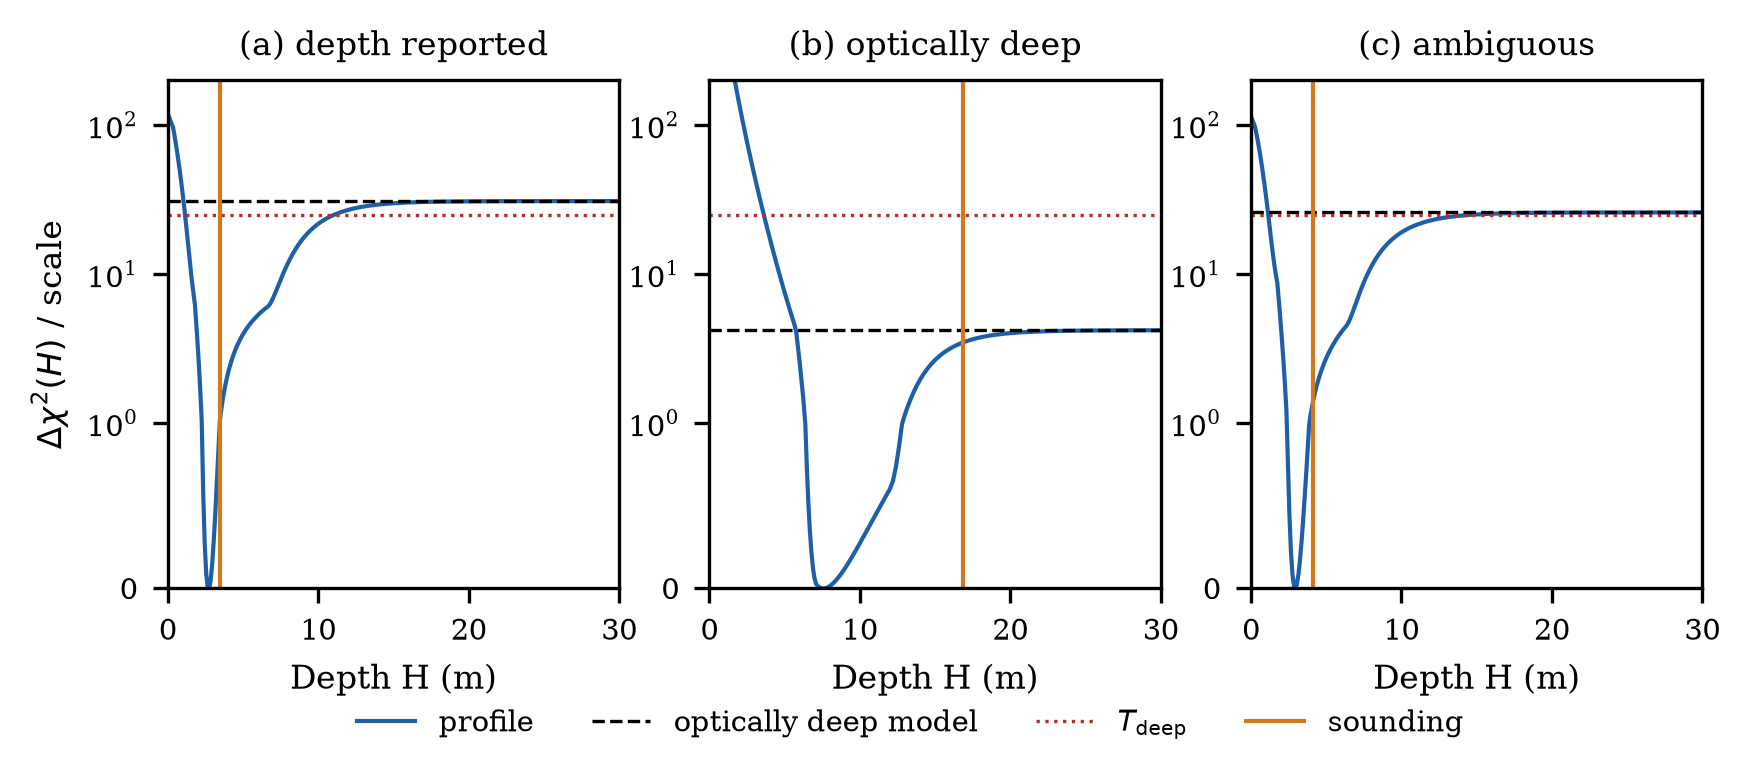
\includegraphics[width=\textwidth]{msab_figures/profiles.png}
\caption{Profile misfit $\Delta\chi^2_p(H) = \chi^2_p(H) - \chi^2_\mathrm{min}$, divided by the scale $q$, for three cells at Bundegi (logarithmic above 1). The dashed line is the optically deep model, the dotted line $T_\mathrm{deep}$, and the orange line the sounded depth. (\textbf{a})~Sounded at 3.45\,m: depth 2.71\,m reported, and the deep model is worse by 31. (\textbf{b})~Sounded at 16.8\,m: the profile's minimum is at 7.5\,m, but the deep model is worse by only 4, so the cell is flagged optically deep and no wrong depth is reported. (\textbf{c})~Sounded at 4.15\,m: the minimum is at 2.9\,m, but depths outside the tolerance band fit within $T_\mathrm{amb}$ of it, so the cell is flagged ambiguous.\label{fig:profiles}}
\end{figure}

\subsection{Assumptions}\label{sec:assumptions}

The model makes the following assumptions. Each is a possible cause of failure, and Section~\ref{sec:discussion} returns to the ones that matter at Exmouth.
\begin{enumerate}[label=A\arabic*.]
\item \textbf{Forward model.} Lee's model~(\ref{eq:lee})--(\ref{eq:u}) describes subsurface reflectance over a homogeneous water column and a Lambertian bottom. Its error relative to exact radiative transfer is represented by a relative error $\varepsilon$ that is independent between bands and scenes.
\item \textbf{Constant seabed.} Depth below the datum and the bottom (class and brightness) are the same in every scene. Scene water depths differ only by the tide $h_s$, which is known from a gauge.
\item \textbf{Locally uniform water.} Within a scene, the water at a pixel has the same inherent optical properties as the optically deep water within $R = 1.5$\,km, and is vertically homogeneous.
\item \textbf{Deep water is present and identifiable.} The window contains optically deep pixels, and they are the darkest in smoothed red and then green. Where a window has too few valid pixels (under 400), the scene-wide reference is used instead.
\item \textbf{QAA.} At 665\,nm absorption is that of pure water. The particle backscatter slope $Y$ follows QAA's empirical relation, and $\kappa = a + b_b$.
\item \textbf{Bottom.} The bottom is one of three spectral shapes with brightness in its class range. Mixtures and other bottom types are represented only to the extent that one of the three shapes fits them.
\item \textbf{Residual correction errors.} Errors left by the atmospheric and glint correction are spectrally flat within a scene, with a standard deviation of $5 \times 10^{-4}$ in $R_\mathrm{rs}$.
\item \textbf{Errors.} Residuals are independent and Gaussian, with variance~(\ref{eq:sigma}).
\item \textbf{Geometry.} Sun and view angles are constant over a site in each scene. Depth lies between 0.05 and 30\,m.
\end{enumerate}

\subsection{Implementation}\label{sec:impl}

The model is implemented in C as \texttt{MODEL Lee\_Profile} in photic~\cite{blake2020}, with the same inputs and outputs as photic's existing semi-analytical model. Each cell gets a depth, its uncertainty, the bottom class and brightness, the misfit, and a flag: depth, optically deep, ambiguous or no data. Smoothed red and green are computed with summed-area tables. Local references are computed once per $8 \times 8$-cell tile, from the deep pixels within $R$ of the tile centre. Per cell, the cost is $O(N_H N_c S L)$ for $N_H = 220$ depths and $N_c = 3$ classes, with no iteration. A Python prototype (\texttt{validation/profile\_model.py}) implements the same model with one reference per cell. On 300 training points, the C port with one reference per cell reproduced the prototype exactly, and the tiled default changed 1 of the 300. Table~\ref{tab:settings} lists the settings.

\begin{table}[H]
\caption{Settings of the profile model. ``Tuned'' settings were chosen on the training split only (Section~\ref{sec:design}).\label{tab:settings}}
\begin{tabularx}{\textwidth}{>{\raggedright\arraybackslash}p{4.2cm}>{\raggedright\arraybackslash}X>{\raggedright\arraybackslash}p{3.2cm}}
\toprule
\textbf{Setting} & \textbf{Value} & \textbf{Source}\\
\midrule
Bands & 443, 492, 560, 665\,nm & Sentinel-2 bands 1--4\\
Deep-water window radius $R$ & 1.5\,km (scene-wide if under 400 valid cells) & tuned\\
Deep-pixel selection & lowest 20\% red, then lowest 15\% green, $7\times7$ smoothing & tuned\\
Relative model error $\varepsilon$ & 0.05 & tuned (tier 2 gives 0.024 median)\\
Optically deep threshold $T_\mathrm{deep}$ & 25 & tuned\\
Ambiguity threshold $T_\mathrm{amb}$ & 1 & tuned\\
Offset prior $\sigma_g$ & $5\times10^{-4}$ in $R_\mathrm{rs}$ & photic's glint offset prior\\
Brightness ranges $[b^-_c, b^+_c]$ & sand 0.15--0.75; seagrass 0.03--0.15; coral 0.03--0.25 & in situ spectra~\cite{roelfsema2012,roelfsema2016}\\
Depth grid & 220 depths, 0.05--30\,m & fixed\\
\bottomrule
\end{tabularx}
\end{table}

\section{Case Study and Validation Design}\label{sec:data}

\subsection{Exmouth Gulf}\label{sec:site}

Exmouth Gulf in north-west Western Australia is a shallow, mostly turbid embayment east of the North West Cape. Its western shore is fringed by sand, seagrass and reef flats. West of the cape, the Ningaloo coast has clear oceanic water over a coral lagoon. We use four sites (Figure~\ref{fig:site}, Table~\ref{tab:sites}):
\begin{itemize}
\item \textbf{Marina:} sand and seagrass flats in the gulf, 0--13\,m;
\item \textbf{Gulf entrance:} mostly 10--24\,m of turbid water, with shoals;
\item \textbf{Bundegi:} the gulf's north-western shore, 0--21\,m;
\item \textbf{Tantabiddi:} the Ningaloo lagoon and reef, 0--28\,m.
\end{itemize}
The first two are the training sites; Bundegi and Tantabiddi are held out. Tantabiddi tests transfer to a different water mass.

\begin{figure}[H]
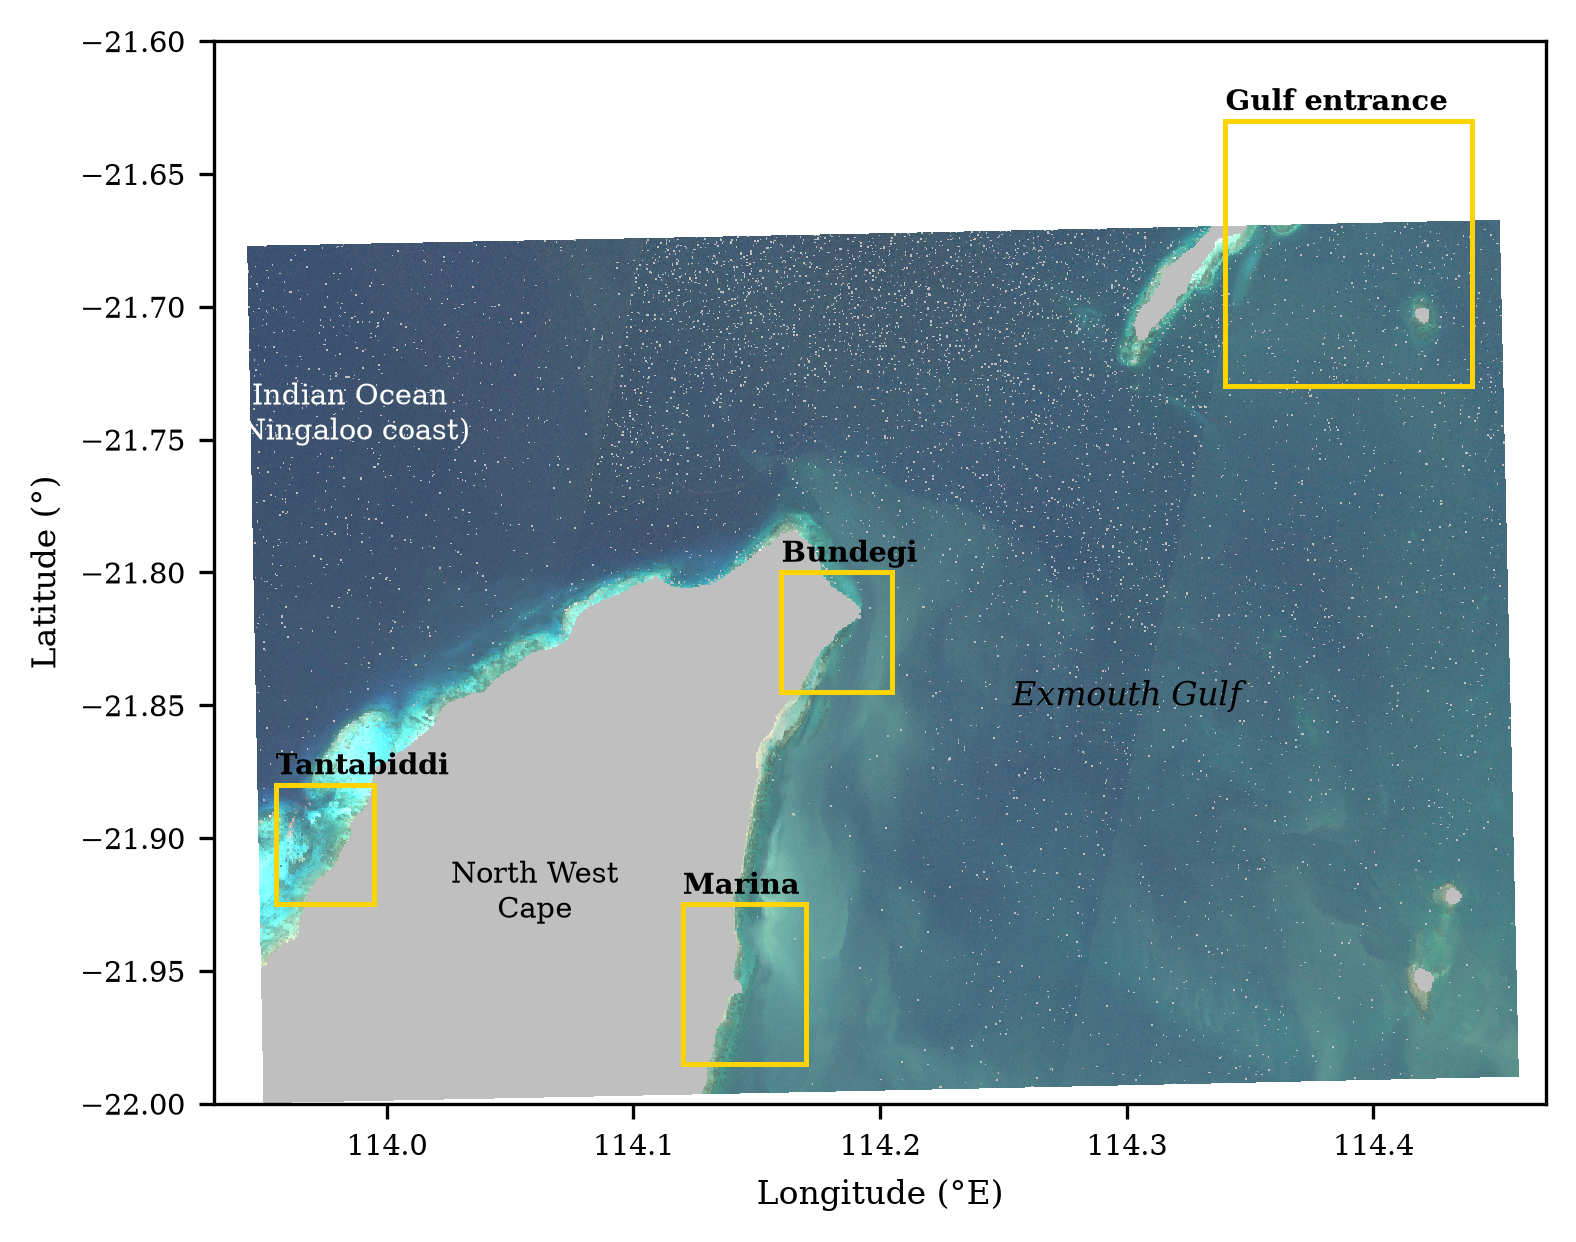
\includegraphics[width=0.8\textwidth]{msab_figures/study_area.png}
\caption{The four validation sites in Exmouth Gulf and on the Ningaloo coast, over a Sentinel-2 true-colour composite (28 April 2019, ACOLITE $R_\mathrm{rs}$; land in grey). Marina and the gulf entrance are the training sites, and Bundegi and Tantabiddi are held out.\label{fig:site}}
\end{figure}

\subsection{Imagery}\label{sec:imagery}

We used six cloud-free Sentinel-2 Level-1C scenes of tile 49KHR (Table~\ref{tab:scenes}), with sun elevations of 37--56$^\circ$ to limit sun glint. They were atmospherically corrected with ACOLITE's dark spectrum fitting with residual glint correction~\cite{vanhellemont2018,vanhellemont2019} at 20\,m. The water-leaving $R_\mathrm{rs}$ was resampled to a regular WGS84 grid of 0.0002$^\circ$ (about 21\,m; 0.0006$^\circ$ at the gulf entrance). Scenes covering less than half as much of a site as the best scene (swath edges) were dropped there, leaving five scenes at Bundegi, four at Tantabiddi and six at Marina and the gulf entrance. Tides at each overpass come from the WA Department of Transport Exmouth tide gauge, as departures from its long-term mean. Depths are relative to mean sea level, which is taken equal to the Australian Height Datum (the difference is under 0.1\,m).

\begin{table}[H]
\caption{Sentinel-2 scenes. Angles are in air; the tide is relative to mean sea level.\label{tab:scenes}}
\begin{tabularx}{\textwidth}{lCCCl}
\toprule
\textbf{Date} & \textbf{Sun zenith} & \textbf{View zenith} & \textbf{Tide (m)} & \textbf{Sites}\\
\midrule
2019-04-28 & 43.1$^\circ$ & 9.5$^\circ$ & $+0.02$ & all\\
2019-06-12 & 51.2$^\circ$ & 9.5$^\circ$ & $-0.34$ & all\\
2021-07-23 & 50.7$^\circ$ & 8.2$^\circ$ & $+0.74$ & all but Tantabiddi\\
2021-09-14 & 34.3$^\circ$ & 9.5$^\circ$ & $-0.72$ & all but Bundegi\\
2022-07-08 & 52.5$^\circ$ & 8.1$^\circ$ & $-0.26$ & all but Tantabiddi\\
2024-06-20 & 51.7$^\circ$ & 9.5$^\circ$ & $+0.62$ & all\\
\bottomrule
\end{tabularx}
\end{table}

\subsection{Reference Depths}\label{sec:reference}

Reference depths come from WA Department of Transport singlebeam surveys (relative to AHD, CC BY 4.0), gridded to the image grid. Each cell takes the median of the most recent survey covering it. Cells with fewer than three soundings or a spread above 0.5\,m are excluded, because they are steep or mixed. Table~\ref{tab:sites} summarises the reference cells. For comparison we also score the published photic Exmouth Gulf product (30\,m). That product was made with photic's original model and an empirical depth prior calibrated with soundings, so it is not a sounding-free result.

\begin{table}[H]
\caption{Validation sites. The share of reference cells in each depth bin is given as 0--5\,m / 5--10\,m / over 10\,m.\label{tab:sites}}
\begin{tabularx}{\textwidth}{lCCCCl}
\toprule
\textbf{Site} & \textbf{Role} & \textbf{Reference cells} & \textbf{Median depth (m)} & \textbf{Range (m)} & \textbf{Depth bins (\%)}\\
\midrule
Marina & training & 9804 & 4.0 & 0.0--13.0 & 62 / 23 / 14\\
Gulf entrance & training & 4171 & 14.7 & 1.4--23.9 & 4 / 3 / 93\\
Bundegi & held out & 2267 & 3.7 & 0.4--20.7 & 72 / 9 / 18\\
Tantabiddi & held out & 11211 & 3.3 & 0.0--28.4 & 76 / 13 / 11\\
\bottomrule
\end{tabularx}
\end{table}

\subsection{Validation Benchmark}\label{sec:validation}

The model was judged with photic's four-tier benchmark (repository directory \texttt{validation/}). Each tier isolates one source of error:
\begin{itemize}
\item \textbf{Tier 1:} checks the C forward model against an independent Python implementation written from the published equations, and against SAMBUCA~\cite{wettle2006}.
\item \textbf{Tier 2:} compares Lee's model with exact radiative transfer from OSOAA~\cite{chami2015}, run in scalar mode with a black and a sky-lit atmosphere. It covers 1,098 combinations of depth, water type, bottom, sun angle and band.
\item \textbf{Tier 3:} inverts synthetic $32 \times 32$ multi-scene images generated by OSOAA. Depth rises from 0.8 to 25\,m down the image, and the bottom is sand, seagrass and coral in vertical strips. There are three water types (clear, moderate and turbid), 1, 2 or 4 scenes with tides of up to 0.8\,m, and noise of 0 or $5\times10^{-4}$ in $R_\mathrm{rs}$. Bottom brightness is either uniform (0.6 for every class) or realistic (sand 0.5, seagrass 0.07, coral 0.10). Some scenarios add an empirical depth prior, and controls are generated with photic's own forward model.
\item \textbf{Tier 4:} the Exmouth Gulf sites above.
\end{itemize}

\subsection{Metrics}\label{sec:metrics}

A depth is within tolerance if $|H - H_\mathrm{ref}| \le 0.5\,\mathrm{m} + 0.1\,H_\mathrm{ref}$. Over the reference cells of a site or scenario we report:
\begin{itemize}
\item the \emph{coverage} (the share of cells given a depth);
\item the share of covered cells within tolerance;
\item \emph{hits}: the share of all reference cells given a depth within tolerance, i.e.\ coverage times the share within tolerance;
\item RMSE, bias and median absolute error on the covered cells.
\end{itemize}
Hits is the headline metric. It rewards a model for giving correct depths, and not for withholding difficult ones. Uncertainties are checked by the share of covered cells with $|H - H_\mathrm{ref}| \le \sigma_H$, which should be about 68\%.

\subsection{Development Protocol}\label{sec:design}

The model was developed in stages, with a decision rule for each stage written down before it ran:
\begin{itemize}
\item \textbf{Screen.} Design choices were screened on a fixed, depth-stratified sample of 300 points, drawn from the training split: tier 3 clear and moderate water, and the Marina and gulf entrance sites. The profile model and photic's semi-analytical model at the same commit were scored on the same points. The net score is hits minus misses (depths outside tolerance) over all points. Its 95\% interval comes from a paired bootstrap~\cite{efron1993}.
\item \textbf{Gate G1 (identifiability).} The model with the water taken from the soundings had to beat the semi-analytical model on the training split. If it could not, the data could not support depth on these scenes.
\item \textbf{Tuning and confirmation.} The deep-pixel rule, $\varepsilon$, $T_\mathrm{deep}$, $T_\mathrm{amb}$, the window radius and the optional components were tuned on the training split. The chosen setting was then confirmed with a second random sample.
\item \textbf{Gate G2 (held-out test).} The frozen model was run once on the test split: tier 3 turbid water, Bundegi and Tantabiddi. It had to give a better net score with no material RMSE regression.
\item \textbf{Full benchmark.} The C implementation was then run on every cell of tiers 3 and 4.
\end{itemize}
The reference throughout is photic's semi-analytical model (\texttt{Lee\_Semi\_Analytical}) at commit d9d14d6. That version already includes the bounded Levenberg--Marquardt search, the class-bounded bottom and an optically deep test, and runs without a depth prior.

\section{Results}\label{sec:results}

\subsection{Forward Model Accuracy}\label{sec:t2}

Tier 1 passed: the C forward model matches the independent implementation to rounding error. In tier 2, Lee's model differs from OSOAA by a median of 2.4\% (95th percentile 6.7\%) under a black sky, and 2.1\% (6.6\%) with an aerosol optical thickness of 0.1. The error is systematic rather than random. It depends on sun angle, from $+2.2\%$ at $\theta_w = 15^\circ$ to $-1.2\%$ at $40^\circ$, and is larger in deep water, from $+4.9\%$ to $-2.0\%$. This motivates the relative model error $\varepsilon$ in~(\ref{eq:sigma}). It also explains why a model whose water parameters are free absorbs this error into them.

\subsection{Diagnosis of the Joint Inversion}\label{sec:intro-diag}

At Marina, the semi-analytical model put depths of 1--10\,m at 0.8--2.3\,m, with a near-black bottom (albedo 0.03--0.05). Two of the six scenes held a water parameter on its bound. Given the true depth as its start, the model reached a relative misfit of 5.2\%, against 5.1\% at the wrong shallow depth. Several attempts to rescue the joint inversion changed little:
\begin{itemize}
\item adding the 705\,nm band;
\item tying the water between scenes;
\item a sediment-only bottom;
\item larger or smaller windows;
\item ten more scenes;
\item rules for choosing scenes;
\item a test that rejects depths with a nearby alternative.
\end{itemize}
None changed the net score by more than about ten points with an interval excluding zero on both splits.

\subsection{Identifiability and Development}\label{sec:dev}

\paragraph{Gate G1.} With the deep-water reference taken from the sounded cells deeper than the bottom's visibility, the profile model beat the semi-analytical model on the training split's tier 4 points. The net score was $+18.7$ points (95\% interval $+8.0$ to $+30.7$), hits rose from 9\% to 21\%, and RMSE on the commonly covered points fell from 2.88 to 1.29\,m. Depth is therefore identifiable on these scenes once the water is right. The flat misfit came from letting the water bend, not from the data. On tier 3 the oracle model's net score was $-3$ points (interval spanning zero), with 43\% lower RMSE.

\paragraph{Water from the image.} The first sounding-free rule, which took the lowest raw red, failed (tier 3 net $-65$ points). In clear water the red reflectance ($\approx 2\times10^{-4}$) is below the noise ($5\times10^{-4}$), so the rule picked noise extremes. Smoothing, the two-stage red-then-green ranking and the local 1.5\,km window fixed this. Table~\ref{tab:tuning} shows the main steps of tuning.

\begin{table}[H]
\small
\caption{Tuning on the training split (300 points, seed 1): tier 4 / tier 3. The semi-analytical model has hits 9 / 23\% and misses 21 / 15\% on these points. RMSE change is on commonly covered points. The chosen setting is in bold.\label{tab:tuning}}
\begin{tabularx}{\textwidth}{>{\raggedright\arraybackslash}Xcccc}
\toprule
\textbf{Setting} & \textbf{Net (pts)} & \textbf{Hits (\%)} & \textbf{Misses (\%)} & \textbf{RMSE change (\%)}\\
\midrule
site-wide water, $\varepsilon$ 0.03, $T_\mathrm{deep}$ 9 & $-11.3$ / $+8.7$ & 17 / 46 & 41 / 29 & $-37$ / $-52$\\
1.5\,km water, $\varepsilon$ 0.03, $T_\mathrm{deep}$ 9 & $-1.3$ / $+8.7$ & 19 / 46 & 33 / 29 & $-45$ / $-52$\\
\quad $T_\mathrm{deep}$ 25 & $+11.3$ / $+9.3$ & 15 / 44 & 17 / 27 & $-41$ / $-52$\\
\quad $T_\mathrm{deep}$ 25, offset $d_s$ & $+16.7$ / $+4.7$ & 19 / 41 & 15 / 28 & $-40$ / $-47$\\
\quad $T_\mathrm{deep}$ 25, 705\,nm band & $+6.0$ / $+9.3$ & 12 / 44 & 19 / 27 & $-49$ / $-52$\\
\quad $T_\mathrm{deep}$ 25, $\varepsilon$ 0.05, $T_\mathrm{amb}$ 1 & $+17.3$ / $+15.3$ & 16 / 35 & 11 / 11 & $-61$ / $-52$\\
\quad \textbf{$T_\mathrm{deep}$ 25, $\varepsilon$ 0.05, $T_\mathrm{amb}$ 1, offset} & $\mathbf{+19.3}$ / $\mathbf{+14.0}$ & \textbf{18 / 32} & \textbf{11 / 10} & $\mathbf{-39}$ / $\mathbf{-52}$\\
\quad $T_\mathrm{deep}$ 25, $\varepsilon$ 0.03, $T_\mathrm{amb}$ 4 & $+18.0$ / $+14.0$ & 7 / 23 & 1 / 1 & $-93$ / $-82$\\
\bottomrule
\end{tabularx}
\end{table}

On a second training sample (seed 2), the chosen setting gave a tier 4 net score of $+20.0$ (interval $+10.0$ to $+30.0$). Hits rose from 9\% to 20\% and misses fell from 19\% to 10\%. The tier 3 net score was $+8.7$, with an interval spanning zero.

\paragraph{Gate G2.} On the held-out split, run once with the settings frozen, the overall net score was $+8.7$ points (95\% interval $+1.0$ to $+16.7$), with RMSE 20\% lower at the same coverage. The tiers moved in the same direction, but neither was significant alone:
\begin{itemize}
\item \textbf{Tier 4:} net $+9.3$; hits rose from 10\% to 17\%, misses fell from 21\% to 19\%, and RMSE fell from 2.76 to 2.19\,m. Bundegi improved clearly ($+14.7$, interval $+2.7$ to $+28.0$), while Tantabiddi was unchanged within the noise ($+4.0$).
\item \textbf{Tier 3 turbid water:} net $+8.0$; misses fell from 11\% to 5\%.
\end{itemize}

\subsection{Exmouth Gulf, All Cells}\label{sec:t4}

Table~\ref{tab:t4} and Figures~\ref{fig:maps}--\ref{fig:bins} give the full tier 4 results. Neither model used soundings or a depth prior.

\begin{table}[H]
\caption{Tier 4, every reference cell. SA: photic's semi-analytical model; Profile: this paper; Published: the published photic product, calibrated with soundings. Coverage, within tolerance (Tol.) and hits are in \%; RMSE and bias are in m.\label{tab:t4}}
\begin{adjustwidth}{-\extralength}{0cm}
\begin{tabularx}{\fulllength}{llCCCCCCC}
\toprule
\textbf{Site} & \textbf{Model} & \textbf{Coverage} & \textbf{Tol.} & \textbf{Hits} & \textbf{Hits 0--5\,m} & \textbf{RMSE} & \textbf{Bias} & \textbf{Run time (s)}\\
\midrule
\multirow{3}{*}{Bundegi} & SA & 22.0 & 41.8 & 9.2 & 12 & 2.39 & $-0.48$ & 2404\\
 & Profile & 30.1 & 71.6 & \textbf{21.6} & 30 & 1.68 & $-0.86$ & 7\\
 & Published & 83.3 & 41.9 & 34.9 & 34 & 3.67 & $+0.64$ & --\\
\midrule
\multirow{3}{*}{Tantabiddi} & SA & 48.9 & 47.5 & 23.2 & 29 & 2.51 & $+0.42$ & 4650\\
 & Profile & 78.8 & 68.8 & \textbf{54.3} & 71 & 2.17 & $-0.54$ & 6\\
 & Published & \multicolumn{7}{c}{outside the published product}\\
\midrule
\multirow{3}{*}{Marina} & SA & 37.3 & 15.9 & 5.9 & 9 & 2.41 & $-2.00$ & 5242\\
 & Profile & 34.6 & 60.4 & \textbf{20.9} & 33 & 3.01 & $-1.81$ & 14\\
 & Published & 90.4 & 67.7 & 61.2 & 43 & 0.97 & $-0.11$ & --\\
\midrule
\multirow{3}{*}{Gulf entrance} & SA & 2.0 & 30.6 & 0.6 & 13 & 4.26 & $-0.92$ & 1232\\
 & Profile & 3.6 & 40.8 & \textbf{1.5} & 33 & 3.85 & $-2.77$ & 3\\
 & Published & 100.0 & 49.6 & 49.6 & 62 & 2.18 & $+1.94$ & --\\
\bottomrule
\end{tabularx}
\end{adjustwidth}
\end{table}

\paragraph{Against the semi-analytical model.} The profile model gives more correct depths at every site, with no soundings and no prior. Hits rose from 9.2\% to 21.6\% at Bundegi, from 23.2\% to 54.3\% at Tantabiddi and from 5.9\% to 20.9\% at Marina. RMSE fell at the two held-out sites, and the profile model runs in 3--14\,s per site against 20--90 minutes. At Marina, coverage was similar but the share within tolerance rose from 16\% to 60\%. RMSE rose there, from 2.41 to 3.01\,m, because cells at 10--13\,m were placed at 4--5\,m. The semi-analytical model instead put almost every Marina depth at 0.8--2.3\,m (Figure~\ref{fig:scatter}). At the gulf entrance, 93\% of the cells are deeper than 10\,m in turbid water. The profile model flags 63\% of them optically deep and 33\% have no valid data, so it gives few depths, as the physics requires (Figure~\ref{fig:maps}).

\paragraph{The depth ceiling.} Almost all the gains are at 0--5\,m. Between 5 and 10\,m the profile model's hits are 0--4\% at every site, and below 10\,m they are 0\%. Fewer than 5\% of its depths exceed 5\,m (Figures~\ref{fig:scatter} and~\ref{fig:bins}). Deeper cells are either flagged optically deep or reported at 3--5\,m, with biases of $-3.0$ to $-4.2$\,m in the 5--10\,m bin and $-6.5$ to $-8.4$\,m in the 10--20\,m bin. The ambiguity test does not catch these cases because their profiles have a clear minimum, but in the wrong place.

At Tantabiddi, cells sounded at 3--5, 5--8 and 8--12\,m all had their profile minimum at 3.9--4.2\,m. Scaling $\kappa$ by 0.7 or 0.5 moved all three groups deeper together, to about 5.5 and 7.5\,m, without separating them and without changing the misfit. Within this model's error, these four-band spectra therefore do not distinguish a deeper, brighter bottom from a shallower, darker one beyond about 5\,m. On synthetic scenes with realistic bottoms and correct water, the same model recovers 10--20\,m with 89\% of depths within tolerance (Section~\ref{sec:t3}). The ceiling therefore comes from the real scenes and the model's assumptions about them, not from the method itself.

\paragraph{Against the published product.} The published product, made with a sounding-calibrated depth prior, gives far more correct depths: 34.9\% against 21.6\% at Bundegi, and 61.2\% against 20.9\% at Marina. Most of its advantage is in deeper water. At Marina it has 86\% hits in the 5--10\,m bin against 1\% for the profile model. At 0--5\,m the two are comparable: 30\% against 34\% at Bundegi and 33\% against 43\% at Marina. On the cells it covers, the profile model's share within tolerance is higher at Bundegi (72\% against 42\%) but lower at Marina (60\% against 68\%). The cells each model covers differ, so the share within tolerance alone does not compare the two models.

\begin{figure}[H]
\begin{adjustwidth}{-\extralength}{0cm}
\centering
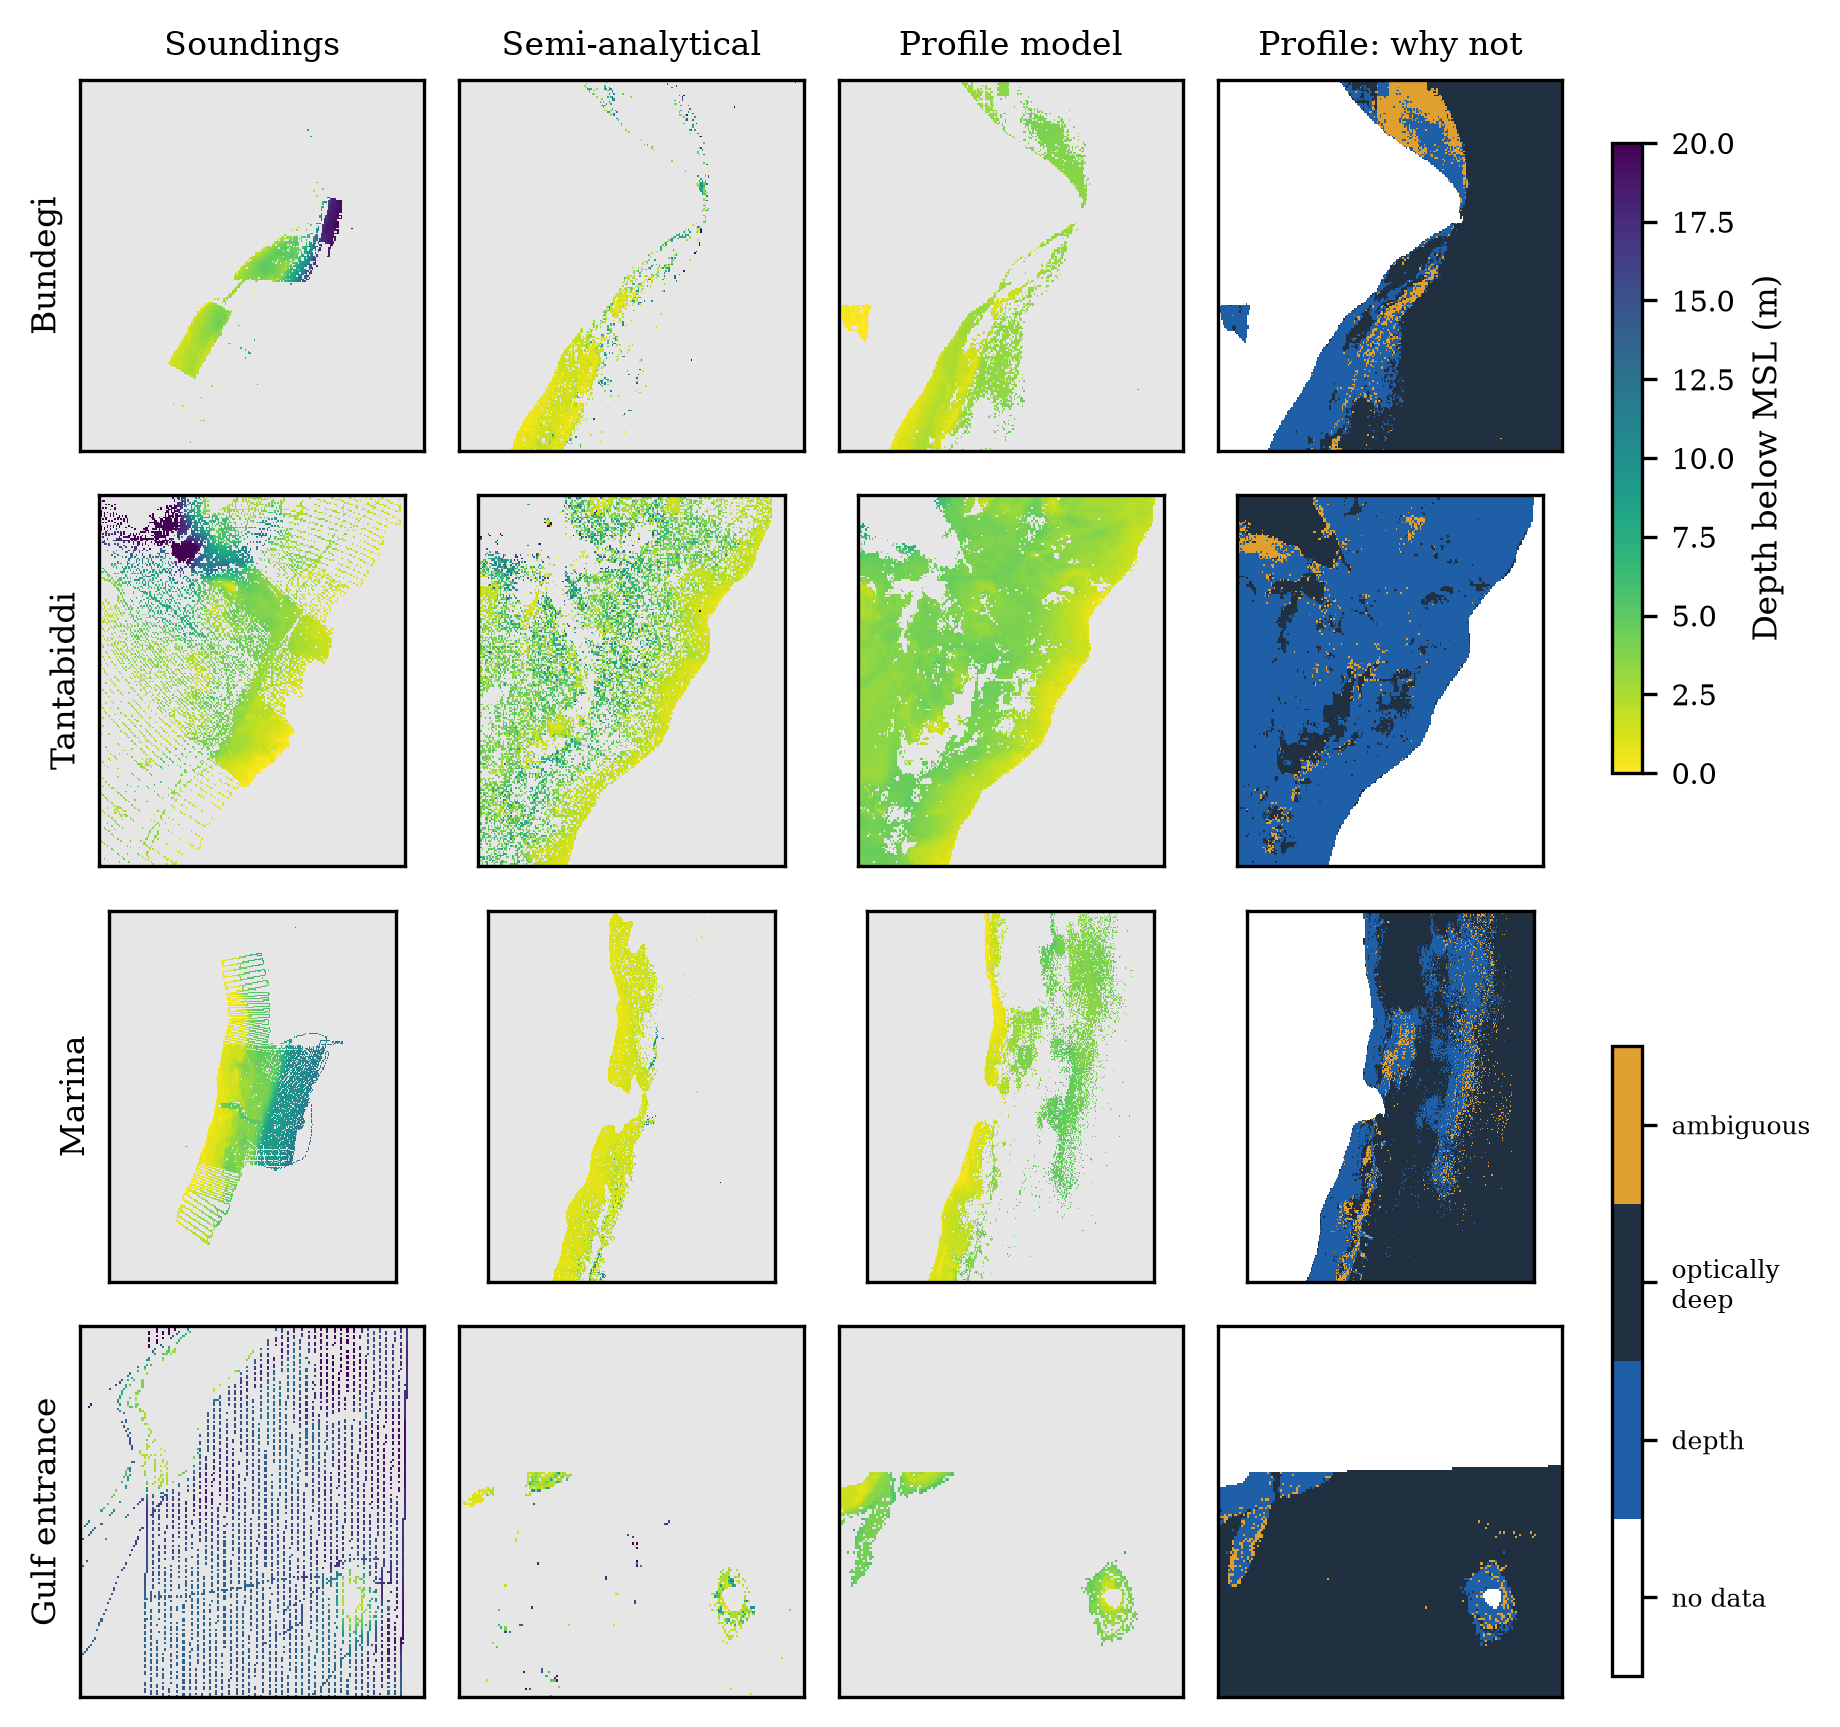
\includegraphics[width=\fulllength]{msab_figures/maps.png}
\end{adjustwidth}
\caption{Reference depths and modelled depths at the four sites: soundings gridded to the image, photic's semi-analytical model, the profile model, and the profile model's flag for each cell (depth, optically deep, ambiguous, or no valid data in enough scenes). Grey: no depth.\label{fig:maps}}
\end{figure}

\begin{figure}[H]
\begin{adjustwidth}{-\extralength}{0cm}
\centering
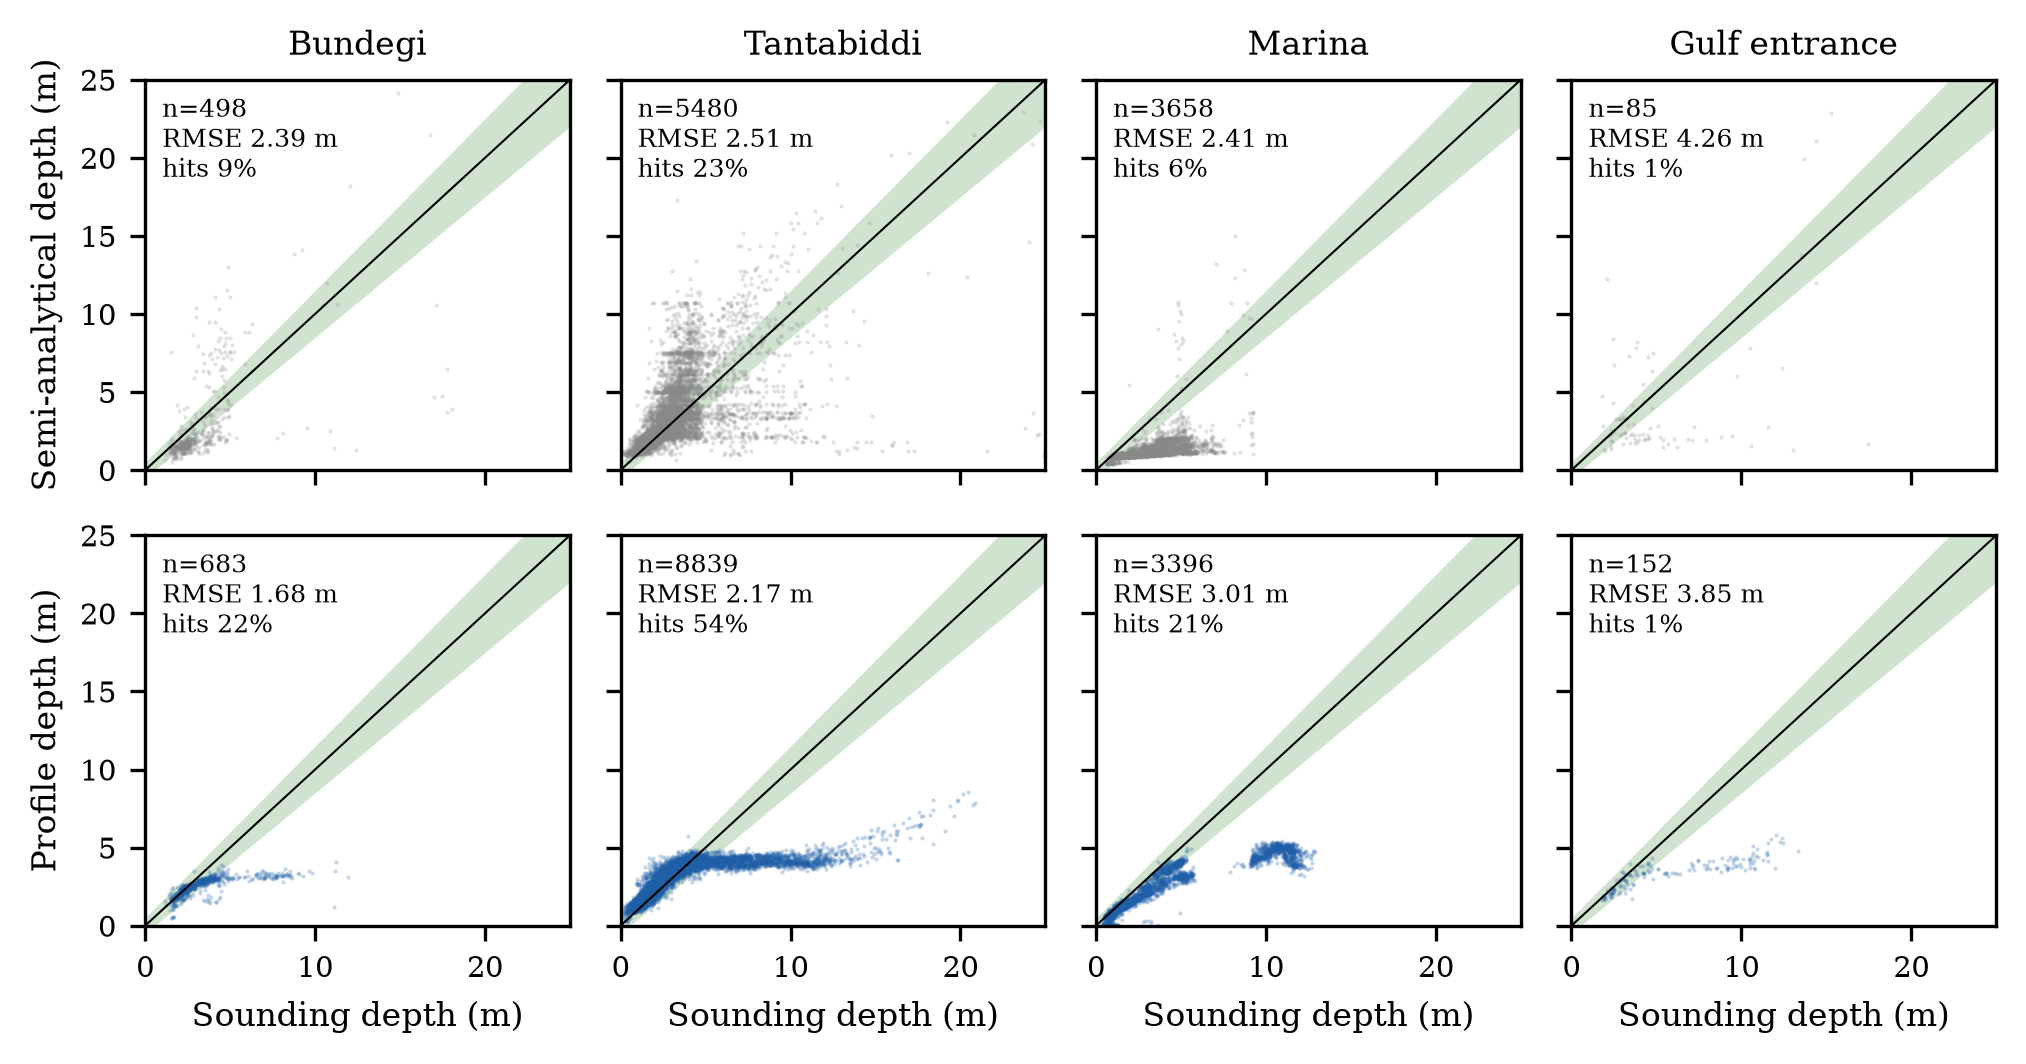
\includegraphics[width=\fulllength]{msab_figures/scatter.png}
\end{adjustwidth}
\caption{Modelled against sounded depth on every covered reference cell. Top: semi-analytical model; bottom: profile model. The green band is the tolerance $0.5 + 0.1H$. Hits are over all reference cells.\label{fig:scatter}}
\end{figure}

\begin{figure}[H]
\begin{adjustwidth}{-\extralength}{0cm}
\centering
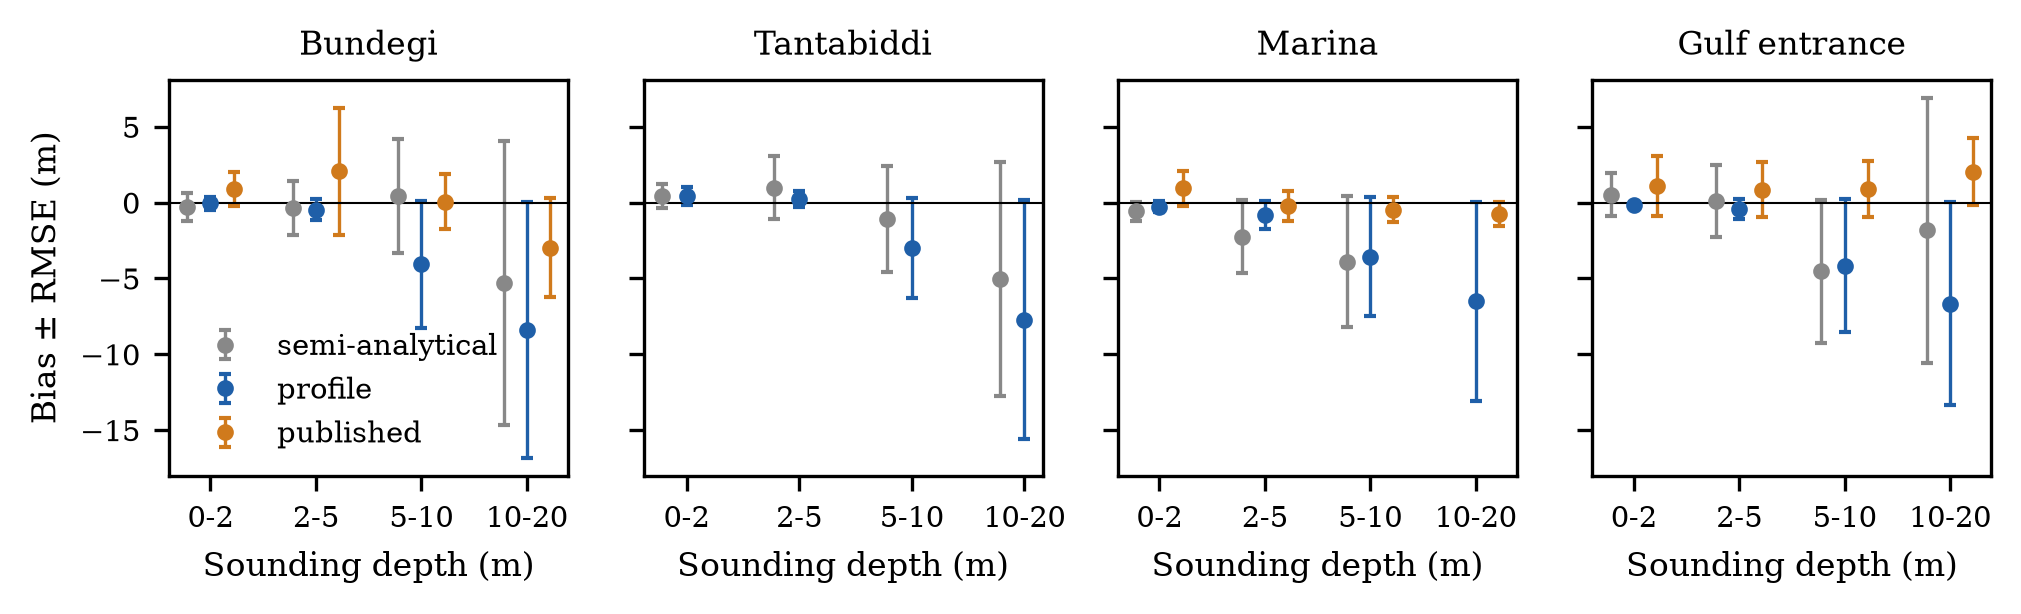
\includegraphics[width=\fulllength]{msab_figures/depth_bins.png}
\end{adjustwidth}
\caption{Bias (points) and RMSE (bars) by sounded depth, for the semi-analytical model, the profile model and the published, sounding-calibrated product.\label{fig:bins}}
\end{figure}

\subsection{Synthetic Scenes}\label{sec:t3}

Table~\ref{tab:t3} and Figure~\ref{fig:t3} summarise tier 3. Where the profile model reports a depth it is usually more accurate. In turbid water the median RMSE is 0.37--0.72\,m against 0.72--2.13\,m, with 84--96\% of depths within tolerance. It abstains more, however, so its hits over all cells are lower on average: 31\% against 46\% in clear water, 16\% against 24\% in moderate water, and 10\% against 13\% in turbid water.

The losses are largest in noise-free scenes. There, the error model ($\varepsilon = 0.05$, tuned for real imagery) is conservative, and the semi-analytical model can bend its water to fit the scenes' own structure. In clear water with noise and realistic bottoms, the profile model doubles the hits (51\% against 24\%) and recovers 10--20\,m with 89\% of depths within tolerance. The profile model ignores the depth prior, so the prior scenarios score as the ones without. In those scenarios the semi-analytical model, drawn away from its prior, has RMSE of 8--14\,m.

\begin{table}[H]
\small
\caption{Tier 3, means over scenarios without a prior (1, 2 and 4 scenes; uniform and realistic bottoms; with and without noise; controls). Hits and coverage in \%, RMSE the median over scenarios in m.\label{tab:t3}}
\begin{tabularx}{\textwidth}{>{\raggedright\arraybackslash}p{2.7cm}CCCCCC}
\toprule
 & \multicolumn{3}{c}{\textbf{Semi-analytical}} & \multicolumn{3}{c}{\textbf{Profile}}\\
\textbf{Water} & \textbf{Coverage} & \textbf{Hits} & \textbf{RMSE} & \textbf{Coverage} & \textbf{Hits} & \textbf{RMSE}\\
\midrule
Clear & 59 & 45.6 & 1.87 & 42 & 31.4 & 1.67\\
Moderate & 38 & 24.1 & 3.20 & 30 & 15.9 & 1.88\\
Turbid & 19 & 12.6 & 1.78 & 13 & 10.1 & 0.65\\
\midrule
Clear, noise, realistic bottoms & 25 & 23.9 & 0.78 & 59 & 50.6 & 1.38\\
\bottomrule
\end{tabularx}
\end{table}

\begin{figure}[H]
\begin{adjustwidth}{-\extralength}{0cm}
\centering
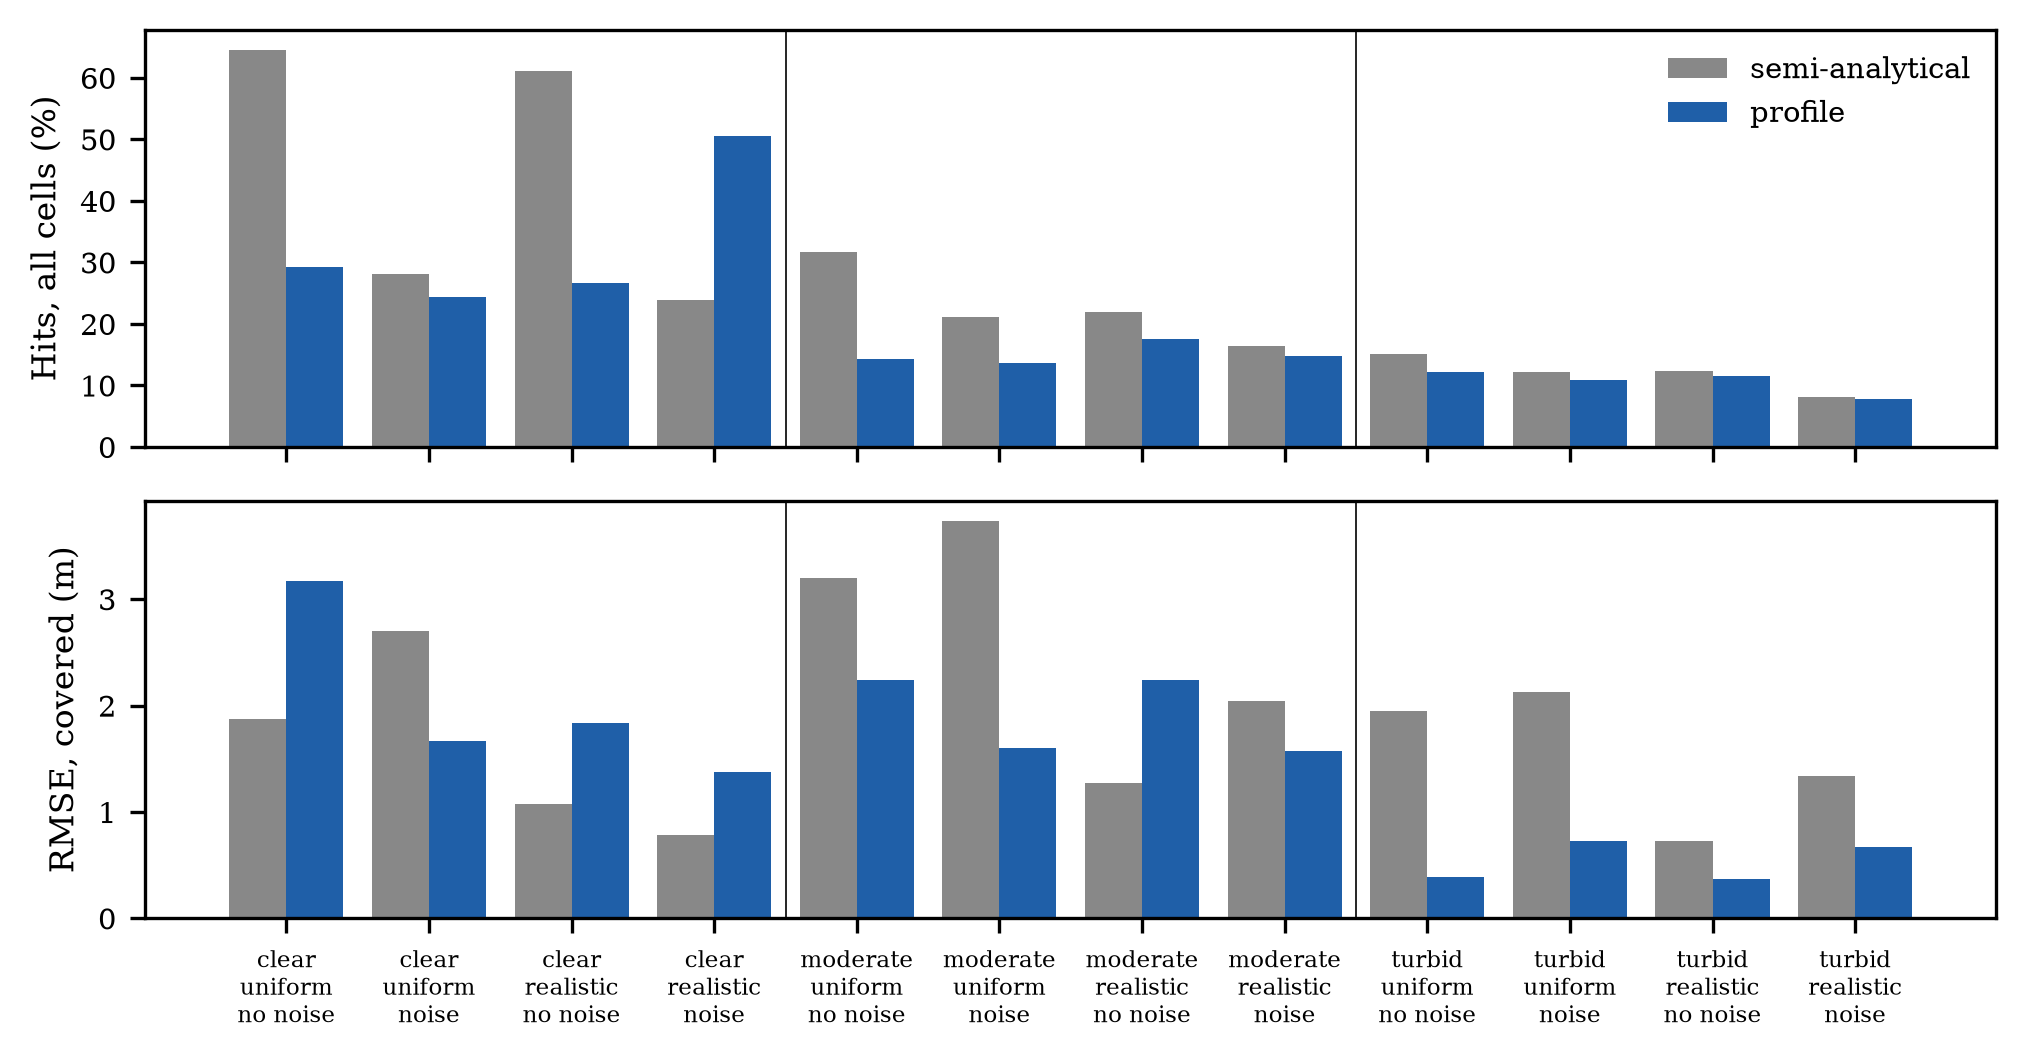
\includegraphics[width=\fulllength]{msab_figures/tier3.png}
\end{adjustwidth}
\caption{Tier 3 by water type, bottom (uniform brightness 0.6, or realistic class brightnesses) and noise ($5\times10^{-4}$ in $R_\mathrm{rs}$), averaged over 1, 2 and 4 scenes. Top: hits over all cells; bottom: RMSE where a depth is given.\label{fig:t3}}
\end{figure}

\subsection{Ablation}\label{sec:ablation}

Because the profile model runs in seconds, every component could be switched off in turn and run on all cells of both tiers (Table~\ref{tab:ablation}). Only the optically deep threshold changes the result substantially. At $T_\mathrm{deep} = 64$ hits fall by half or more at every Exmouth site. At $T_\mathrm{deep} = 9$ coverage rises (Marina 35\% to 64\%), and hits rise by 1--3 points at the cost of higher RMSE.

The other components matter little on the full sites. The scene-wide reference is as good as the 1.5\,km window, slightly better at Tantabiddi and Marina and slightly worse at Bundegi and the gulf entrance. Without the offset, Bundegi loses 2 points and its coverage falls from 30\% to 21\%, while tier 3's clear-water hits rise by 7 points. Without the ambiguity test, hits change by under 2 points while RMSE rises at the held-out sites. The red-only selection loses 8 points at Tantabiddi. Several choices that the 300-point screen favoured are therefore not supported by the full benchmark. A simpler model, with scene-wide water and no offset, would do about as well.

\begin{table}[H]
\small
\caption{Ablation on all cells: hits (\%) at each Exmouth site, and mean hits (\%) over tier 3 scenarios without a prior.\label{tab:ablation}}
\begin{adjustwidth}{-\extralength}{0cm}
\begin{tabularx}{\fulllength}{>{\raggedright\arraybackslash}p{3.8cm}CCCCCCC}
\toprule
\textbf{Variant} & \textbf{Bundegi} & \textbf{Tantabiddi} & \textbf{Marina} & \textbf{Gulf ent.} & \textbf{T3 clear} & \textbf{T3 moderate} & \textbf{T3 turbid}\\
\midrule
Profile model as tuned & 21.6 & 54.3 & 20.9 & 1.5 & 31.4 & 15.9 & 10.1\\
No offset $d_s$ & 19.3 & 56.2 & 20.0 & 1.7 & 38.2 & 20.9 & 7.9\\
Scene-wide water ($R = \infty$) & 20.2 & 56.3 & 23.0 & 1.2 & 31.4 & 15.9 & 10.1\\
No ambiguity test & 22.1 & 55.0 & 22.9 & 1.6 & 43.8 & 19.9 & 11.6\\
$T_\mathrm{deep} = 9$ & 24.9 & 57.8 & 23.8 & 1.5 & 32.1 & 16.3 & 11.3\\
$T_\mathrm{deep} = 64$ & 12.0 & 20.8 & 4.5 & 1.2 & 29.5 & 14.7 & 6.7\\
$\varepsilon = 0.03$ & 20.2 & 53.1 & 21.1 & 1.4 & 30.4 & 15.9 & 11.0\\
No smoothing in deep-pixel selection & 21.0 & 54.6 & 19.6 & 1.1 & 24.2 & 15.8 & 11.2\\
Red-only deep-pixel selection & 20.8 & 45.9 & 18.5 & 1.6 & 23.3 & 15.5 & 9.1\\
\bottomrule
\end{tabularx}
\end{adjustwidth}
\noindent{\footnotesize{The tier 3 scenes span 32 cells (about 10\,m), so the window covers each scene and the scene-wide variant is identical there.}}
\end{table}

\subsection{Number of Scenes}\label{sec:scenes}

We ran the model at each site with every subset of its scenes (Figure~\ref{fig:scenes}). On average, hits rise with the number of scenes, most steeply at Tantabiddi: from 26\% with one scene to 54\% with all four. The spread between subsets is wide. At Marina, single scenes give 0.3--22\% hits and the best three-scene subset gives 36\%, against 21\% with all six. One poor scene can therefore cost more than an extra scene gains. Without soundings, however, the best subset cannot be chosen, and earlier attempts to choose scenes by simple rules did not help (Section~\ref{sec:intro-diag}).

\begin{figure}[H]
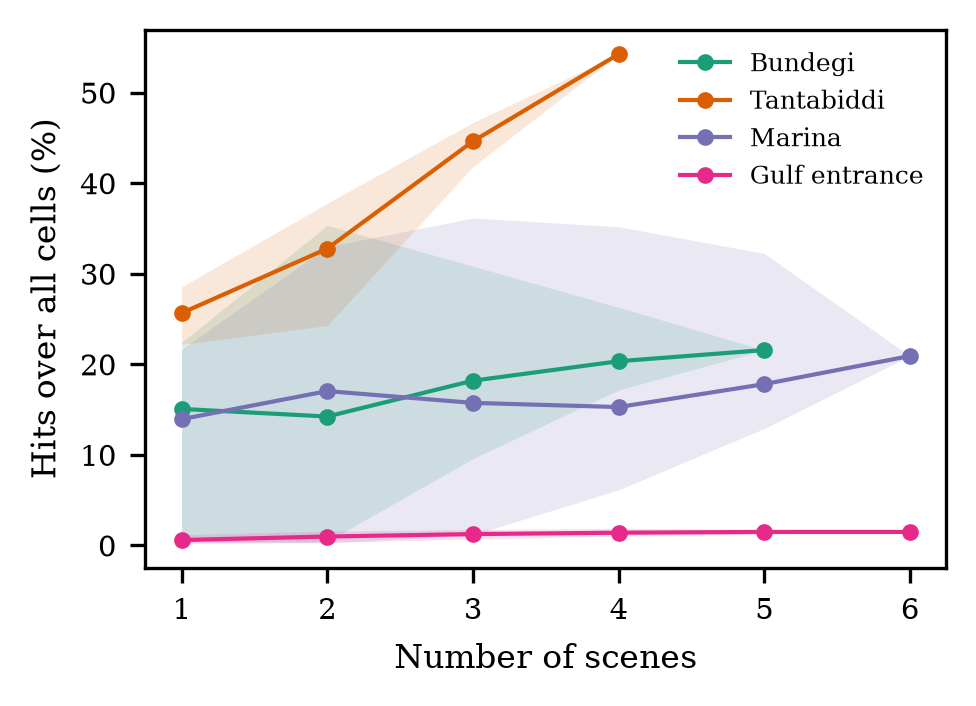
\includegraphics[width=0.55\textwidth]{msab_figures/scenes.png}
\caption{Hits against the number of scenes used, for every subset of each site's scenes: mean (line) and range over subsets (shading).\label{fig:scenes}}
\end{figure}

\subsection{Uncertainty}\label{sec:sigma}

The profile model's $\sigma_H$ is too small, but far better calibrated than the semi-analytical model's. The share of covered cells within $\pm\sigma_H$ of the sounding is 46\%, 35\%, 18\% and 14\% at Bundegi, Tantabiddi, Marina and the gulf entrance, against the nominal 68\%. For the semi-analytical model it is 4\%, 11\%, 0\% and 8\%. The median $\sigma_H$ is 0.25--0.35\,m, against median errors of 0.37--1.6\,m. The underestimate is largest where the depth ceiling acts, as expected: a profile with a clear but displaced minimum gives a narrow $\sigma_H$ around the wrong depth.

\subsection{Deep-Water Reference}\label{sec:refres}

Figure~\ref{fig:reference} shows the deep pixels chosen at Marina and every scene's site-wide deep-water spectrum. The references are consistent within each site. The exception is one Tantabiddi scene (2019-06-12), whose reference is about 50\% brighter: there the darkest red was a clearer water mass over a 4\,m lagoon.

\begin{figure}[H]
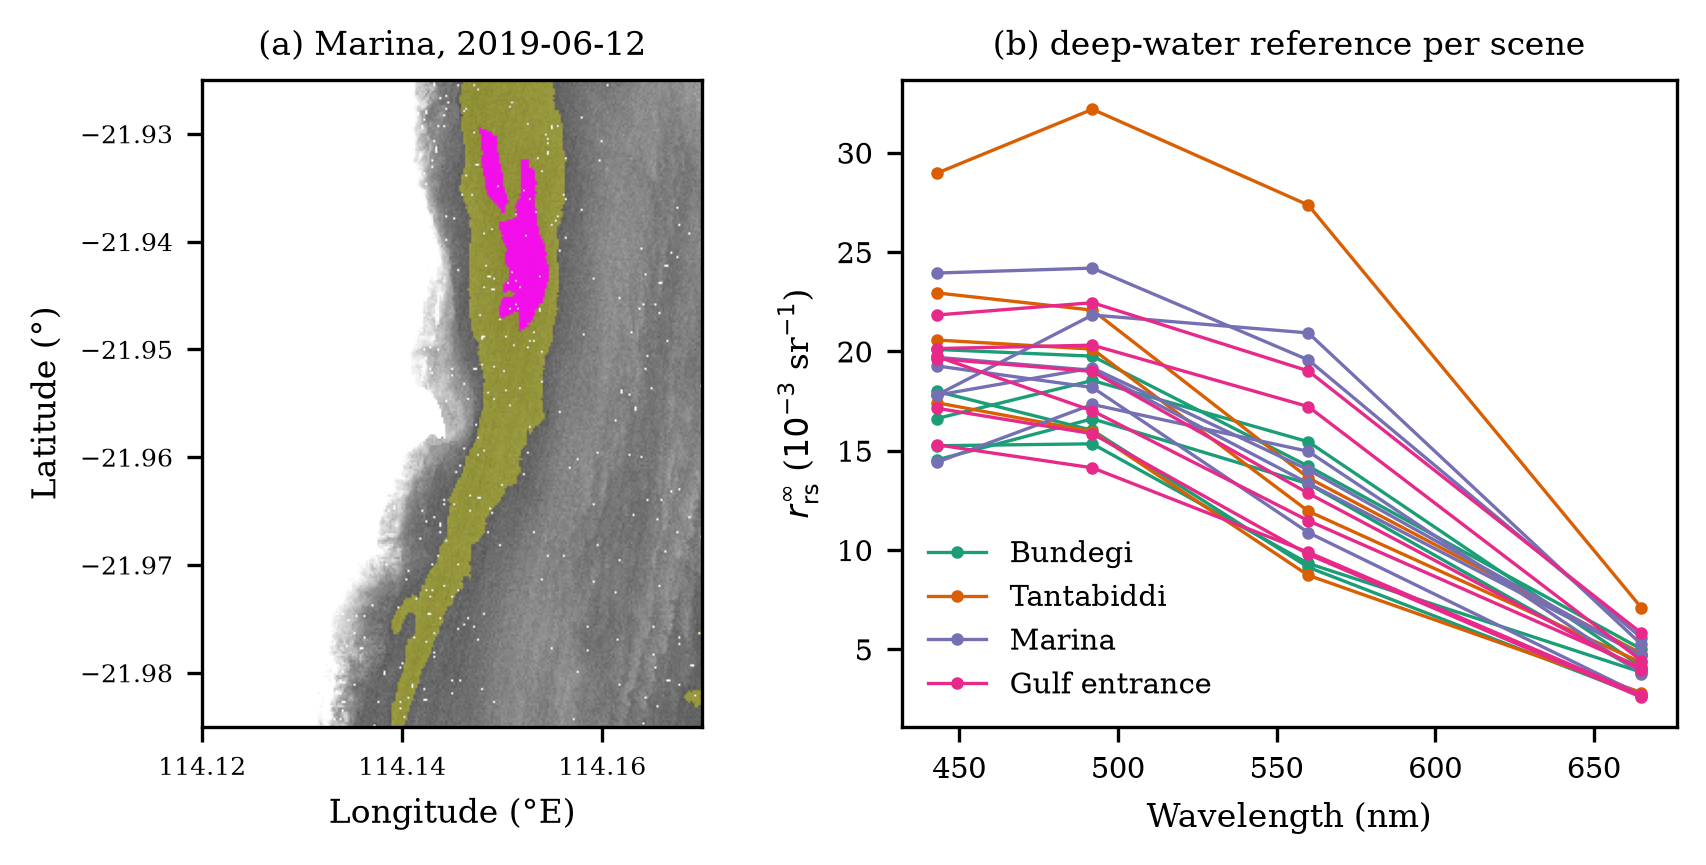
\includegraphics[width=\textwidth]{msab_figures/reference.png}
\caption{(\textbf{a})~Marina, 2019-06-12: red $R_\mathrm{rs}$ (grey), the 20\% of cells darkest in smoothed red (yellow), and the deep cells chosen from them by green (magenta). (\textbf{b})~Site-wide deep-water reflectance of every scene at each site.\label{fig:reference}}
\end{figure}

\section{Discussion}\label{sec:discussion}

\subsection{What Changed and Why It Converges}

The profile model does not change the physics of HOPE. It changes which quantities are estimated and how. Water properties are estimated where they are observable, from optically deep pixels, and not where they trade against depth. The bottom brightness and the scene offsets are solved in closed form. Depth, the one non-linear unknown, is searched exhaustively. The result is reproducible, has no starting values, and has an exact misfit profile from which detectability, ambiguity and uncertainty can all be read.

Gate G1 established the central point: on these Sentinel-2 scenes, depth becomes identifiable once the water is fixed correctly. The same scenes defeated the joint inversion regardless of its start. Converging to the right answer therefore depends less on the optimiser than on removing the freedom that made the misfit flat.

\subsection{Where It Fails}

\paragraph{Depth beyond about 5\,m on real scenes.} This is the main limitation. Figure~\ref{fig:scatter} shows depths saturating at 4--5\,m at Tantabiddi and Marina, although the synthetic tier 3 scenes recover 10--20\,m in clear water. Several assumptions could cause this:
\begin{itemize}
\item \textbf{A3 (uniform water).} The water over the shallows and lagoons may be more turbid, or differently coloured, than the deep reference water.
\item \textbf{A5 (QAA).} QAA's pure-water assumption at 665\,nm, or its backscatter slope, may set the spectral shape of $\kappa$ wrongly.
\item \textbf{A6 (bottom).} Bottoms may darken with depth (sand giving way to seagrass and rubble), and the three class shapes may not span real mixtures.
\item \textbf{A1 (forward model).} The forward model's error grows in the regime where the bottom signal is small.
\end{itemize}
Uniformly scaling $\kappa$ did not separate the depths, so a single calibration factor is not enough. Distinguishing between these causes needs field measurements of attenuation and bottom reflectance, or hyperspectral data, at the sites. Meanwhile the flags, and depths reported only up to about 5\,m, are the honest product of this model on these scenes.

\paragraph{Abstention in clean data.} The thresholds were tuned for real imagery, where $\varepsilon = 0.05$ is realistic. On noise-free synthetic scenes they withhold depths the data support, and hits fall in clear and moderate water. Scaling the thresholds by a noise estimate per scene, which the deep pixels already provide, is the natural remedy. Any such re-tuning needs a fresh held-out sample, because the test split has now been used.

\paragraph{Sounding-calibrated products.} The published product, made with a sounding-calibrated empirical prior, remains far more accurate at 5--20\,m. The profile model does not replace soundings where they are available. A depth prior could be added to the profile as one more term, $(H - H_\mathrm{prior})^2/\sigma_\mathrm{prior}^2$, without losing exactness. It would then combine the prior with the image where the image is informative, and defer to the prior where it is not.

\subsection{Lessons for Validation}

Three lessons from this study apply to other models:
\begin{itemize}
\item \textbf{Score over all cells.} Accuracy on a model's own covered cells rewards abstention and hides failures. Hits over all reference cells, together with a breakdown by depth, exposed the depth ceiling that RMSE and the share within tolerance on covered cells did not show.
\item \textbf{Confirm screened choices on full data.} Several choices favoured by the 300-point screen did not hold up on full sites: the local window gave no gain, and the offset helped at one site only (Table~\ref{tab:ablation}).
\item \textbf{Separate tuning from testing.} The held-out gain (net $+8.7$ points) was smaller than the training gain ($+19$ points), as expected after tuning, but it was still significant.
\end{itemize}

\subsection{Future Work}

Future work, in order of expected gain:
\begin{enumerate}
\item diagnose the depth ceiling with in situ attenuation and bottom data;
\item noise-scaled thresholds;
\item a depth prior term in the profile;
\item a per-scene turbidity factor for shallows that are more turbid than the deep reference;
\item robust per-scene weights;
\item a two-class bottom mixture, which remains linear in the brightnesses and so preserves the exact profile;
\item validation at a second region.
\end{enumerate}

\section{Conclusions}

We derived a semi-analytical bathymetry model for multispectral imagery that observes the water from each scene's optically deep pixels, solves the bottom brightness and scene offsets exactly, and searches depth exhaustively. Its minimum is global by construction. It reports a depth only when the profile excludes both optically deep water and a clearly different depth.

On six Sentinel-2 scenes of Exmouth Gulf it was validated without soundings or a prior, with tuning confined to training sites and a single held-out test. Compared with the previous semi-analytical model, it raised the share of surveyed cells given a correct depth from 9\% to 22\%, from 23\% to 54\% and from 6\% to 21\% at three sites. It also ran about 500 times faster and gave better-calibrated uncertainties. Its gains are confined to 0--5\,m. Deeper bottoms are flagged or reported too shallow, and there a sounding-calibrated product remains more accurate. On synthetic scenes it is more accurate where it reports a depth, but it abstains more than the joint inversion. The model, the benchmark and every result in this paper are reproducible from the photic repository.

\vspace{6pt}

\authorcontributions{Conceptualization, methodology, software, validation, formal analysis, writing---original draft preparation and writing---review and editing, S.B. The author has read and agreed to the published version of the manuscript.}

\funding{This research received no external funding.}

\institutionalreview{Not applicable.}

\informedconsent{Not applicable.}

\dataavailability{Sentinel-2 Level-1C data are available from the Copernicus programme, and were obtained from the public Google Cloud Sentinel-2 bucket. Singlebeam surveys and tide-gauge records are published by the Western Australian Department of Transport under CC BY 4.0. The model (\texttt{model/profile.c}), the prototype, the benchmark and the scripts that produce every table and figure (\texttt{validation/paper\_profile.py}) are available at \url{https://github.com/stblake/photic}. Lee's HOPE spreadsheet, used in tier 1, is not redistributed.}

\acknowledgments{During the preparation of this study and manuscript the author used Claude (Anthropic, Claude Opus 5.5) to implement the model and the benchmark, to run the experiments and to draft the text. The author has reviewed and edited the output and takes full responsibility for the content of this publication.}

\conflictsofinterest{The author declares no conflicts of interest.}

\abbreviations{Abbreviations}{
The following abbreviations are used in this manuscript:\\

\noindent
\begin{tabular}{@{}ll}
AHD & Australian Height Datum\\
HOPE & Hyperspectral Optimisation Process Exemplar\\
IOP & Inherent optical property\\
MAD & Median absolute deviation\\
MSL & Mean sea level\\
OSOAA & Ordres Successifs Oc\'ean Atmosph\`ere Avanc\'e (radiative transfer code)\\
QAA & Quasi-analytical algorithm\\
RMSE & Root-mean-square error\\
SA & Semi-analytical\\
SDB & Satellite-derived bathymetry
\end{tabular}
}

\begin{adjustwidth}{-\extralength}{0cm}

\reftitle{References}

\begin{thebibliography}{999}

\bibitem[Lyzenga(1978)]{lyzenga1978}
Lyzenga, D.R. Passive remote sensing techniques for mapping water depth and bottom features. {\em Appl. Opt.} {\bf 1978}, {\em 17}, 379--383.

\bibitem[Lyzenga et~al.(2006)]{lyzenga2006}
Lyzenga, D.R.; Malinas, N.P.; Tanis, F.J. Multispectral bathymetry using a simple physically based algorithm. {\em IEEE Trans. Geosci. Remote Sens.} {\bf 2006}, {\em 44}, 2251--2259.

\bibitem[Stumpf et~al.(2003)]{stumpf2003}
Stumpf, R.P.; Holderied, K.; Sinclair, M. Determination of water depth with high-resolution satellite imagery over variable bottom types. {\em Limnol. Oceanogr.} {\bf 2003}, {\em 48}, 547--556.

\bibitem[Caballero and Stumpf(2019)]{caballero2019}
Caballero, I.; Stumpf, R.P. Retrieval of nearshore bathymetry from Sentinel-2A and 2B satellites in South Florida coastal waters. {\em Estuar. Coast. Shelf Sci.} {\bf 2019}, {\em 226}, 106277.

\bibitem[Lee et~al.(1998)]{lee1998}
Lee, Z.; Carder, K.L.; Mobley, C.D.; Steward, R.G.; Patch, J.S. Hyperspectral remote sensing for shallow waters. I. A semianalytical model. {\em Appl. Opt.} {\bf 1998}, {\em 37}, 6329--6338.

\bibitem[Lee et~al.(1999)]{lee1999}
Lee, Z.; Carder, K.L.; Mobley, C.D.; Steward, R.G.; Patch, J.S. Hyperspectral remote sensing for shallow waters: 2. Deriving bottom depths and water properties by optimization. {\em Appl. Opt.} {\bf 1999}, {\em 38}, 3831--3843.

\bibitem[Lee et~al.(2001)]{lee2001}
Lee, Z.; Carder, K.L.; Chen, R.F.; Peacock, T.G. Properties of the water column and bottom derived from Airborne Visible Infrared Imaging Spectrometer (AVIRIS) data. {\em J. Geophys. Res.} {\bf 2001}, {\em 106}, 11639--11651.

\bibitem[Mobley et~al.(2005)]{mobley2005}
Mobley, C.D.; Sundman, L.K.; Davis, C.O.; Bowles, J.H.; Downes, T.V.; Leathers, R.A.; Montes, M.J.; Bissett, W.P.; Kohler, D.D.R.; Reid, R.P.; et~al. Interpretation of hyperspectral remote-sensing imagery by spectrum matching and look-up tables. {\em Appl. Opt.} {\bf 2005}, {\em 44}, 3576--3592.

\bibitem[Brando et~al.(2009)]{brando2009}
Brando, V.E.; Anstee, J.M.; Wettle, M.; Dekker, A.G.; Phinn, S.R.; Roelfsema, C. A physics based retrieval and quality assessment of bathymetry from suboptimal hyperspectral data. {\em Remote Sens. Environ.} {\bf 2009}, {\em 113}, 755--770.

\bibitem[Dekker et~al.(2011)]{dekker2011}
Dekker, A.G.; Phinn, S.R.; Anstee, J.; Bissett, P.; Brando, V.E.; Casey, B.; Fearns, P.; Hedley, J.; Klonowski, W.; Lee, Z.P.; et~al. Intercomparison of shallow water bathymetry, hydro-optics, and benthos mapping techniques in Australian and Caribbean coastal environments. {\em Limnol. Oceanogr. Methods} {\bf 2011}, {\em 9}, 396--425.

\bibitem[Wettle and Brando(2006)]{wettle2006}
Wettle, M.; Brando, V.E. {\em SAMBUCA: Semi-Analytical Model for Bathymetry, Un-mixing, and Concentration Assessment}; CSIRO Land and Water Science Report 22/06; CSIRO: Canberra, Australia, 2006.

\bibitem[Klonowski et~al.(2007)]{klonowski2007}
Klonowski, W.M.; Fearns, P.R.C.S.; Lynch, M.J. Retrieving key benthic cover types and bathymetry from hyperspectral imagery. {\em J. Appl. Remote Sens.} {\bf 2007}, {\em 1}, 011505.

\bibitem[Hedley et~al.(2009)]{hedley2009}
Hedley, J.; Roelfsema, C.; Phinn, S.R. Efficient radiative transfer model inversion for remote sensing applications. {\em Remote Sens. Environ.} {\bf 2009}, {\em 113}, 2527--2532.

\bibitem[Hedley et~al.(2018)]{hedley2018}
Hedley, J.D.; Roelfsema, C.; Brando, V.; Giardino, C.; Kutser, T.; Phinn, S.; Mumby, P.J.; Barrilero, O.; Laporte, J.; Koetz, B. Coral reef applications of Sentinel-2: Coverage, characteristics, bathymetry and benthic mapping with comparison to Landsat 8. {\em Remote Sens. Environ.} {\bf 2018}, {\em 216}, 598--614.

\bibitem[Lee and Carder(2002)]{lee2002bands}
Lee, Z.; Carder, K.L. Effect of spectral band numbers on the retrieval of water column and bottom properties from ocean color data. {\em Appl. Opt.} {\bf 2002}, {\em 41}, 2191--2201.

\bibitem[Drusch et~al.(2012)]{drusch2012}
Drusch, M.; Del Bello, U.; Carlier, S.; Colin, O.; Fernandez, V.; Gascon, F.; Hoersch, B.; Isola, C.; Laberinti, P.; Martimort, P.; et~al. Sentinel-2: ESA's optical high-resolution mission for GMES operational services. {\em Remote Sens. Environ.} {\bf 2012}, {\em 120}, 25--36.

\bibitem[Blake(2020)]{blake2020}
Blake, S. A multi-spatial, multi-temporal, semi-analytical model for bathymetry, water turbidity and bottom composition using multispectral imagery. {\em arXiv} {\bf 2020}, arXiv:2002.02298.

\bibitem[Maritorena et~al.(1994)]{maritorena1994}
Maritorena, S.; Morel, A.; Gentili, B. Diffuse reflectance of oceanic shallow waters: Influence of water depth and bottom albedo. {\em Limnol. Oceanogr.} {\bf 1994}, {\em 39}, 1689--1703.

\bibitem[Lee et~al.(2002)]{lee2002qaa}
Lee, Z.; Carder, K.L.; Arnone, R.A. Deriving inherent optical properties from water color: A multiband quasi-analytical algorithm for optically deep waters. {\em Appl. Opt.} {\bf 2002}, {\em 41}, 5755--5772.

\bibitem[Pope and Fry(1997)]{pope1997}
Pope, R.M.; Fry, E.S. Absorption spectrum (380--700 nm) of pure water. II. Integrating cavity measurements. {\em Appl. Opt.} {\bf 1997}, {\em 36}, 8710--8723.

\bibitem[Morel(1974)]{morel1974}
Morel, A. Optical properties of pure water and pure sea water. In {\em Optical Aspects of Oceanography}; Jerlov, N.G., Steemann Nielsen, E., Eds.; Academic Press: London, UK, 1974; pp. 1--24.

\bibitem[Roelfsema and Phinn(2012)]{roelfsema2012}
Roelfsema, C.M.; Phinn, S.R. Spectral reflectance library of benthic cover types, Heron Reef, Australia. PANGAEA, 2012. Available online: \url{https://doi.org/10.1594/PANGAEA.804589} (accessed on 13 October 2026).

\bibitem[Roelfsema et~al.(2016)]{roelfsema2016}
Roelfsema, C.M.; Phinn, S.R.; Joyce, K.E. Spectral reflectance of seagrass and sediment, Moreton Bay, Australia. PANGAEA, 2016. Available online: \url{https://doi.org/10.1594/PANGAEA.864310} (accessed on 13 October 2026).

\bibitem[Wilks(1938)]{wilks1938}
Wilks, S.S. The large-sample distribution of the likelihood ratio for testing composite hypotheses. {\em Ann. Math. Stat.} {\bf 1938}, {\em 9}, 60--62.

\bibitem[Vanhellemont and Ruddick(2018)]{vanhellemont2018}
Vanhellemont, Q.; Ruddick, K. Atmospheric correction of metre-scale optical satellite data for inland and coastal water applications. {\em Remote Sens. Environ.} {\bf 2018}, {\em 216}, 586--597.

\bibitem[Vanhellemont(2019)]{vanhellemont2019}
Vanhellemont, Q. Adaptation of the dark spectrum fitting atmospheric correction for aquatic applications of the Landsat and Sentinel-2 archives. {\em Remote Sens. Environ.} {\bf 2019}, {\em 225}, 175--192.

\bibitem[Chami et~al.(2015)]{chami2015}
Chami, M.; Lafrance, B.; Fougnie, B.; Chowdhary, J.; Harmel, T.; Waquet, F. OSOAA: A vector radiative transfer model of coupled atmosphere-ocean system for a rough sea surface application to the estimates of the directional variations of the water leaving reflectance to better process multi-angular satellite sensors data over the ocean. {\em Opt. Express} {\bf 2015}, {\em 23}, 27829--27852.

\bibitem[Efron and Tibshirani(1993)]{efron1993}
Efron, B.; Tibshirani, R.J. {\em An Introduction to the Bootstrap}; Chapman \& Hall: New York, NY, USA, 1993.

\end{thebibliography}

\end{adjustwidth}
\end{document}
